% 12pt: grandezza carattere
% a4paper: formato a4
% openright: apre i capitoli a destra
% twoside: serve per fare un
% documento fronteretro
% report: stile tesi (oppure book)
\documentclass[12pt,a4paper,openright,twoside]{book}

% libreria per accettare i caratteri
% digitati da tastiera come ?
% si può usare anche
% \usepackage[T1]{fontenc}
% però con questa libreria
% il tempo di compilazione
% aumenta
\usepackage[utf8]{inputenc}

%libreria per scrivere in italiano
\usepackage[italian]{babel}

\usepackage{hyperref}

% libreria per impostare il documento
\usepackage{fancyhdr}

% libreria per avere l'indentazione all'inizio dei capitoli, ...
\usepackage{indentfirst}

%libreria per mostrare le etichette
%\usepackage{showkeys}

% libreria per inserire grafici
\usepackage{graphicx}

% libreria per utilizzare font particolari ad esempio \textsc{}
\usepackage{newlfont}

% librerie matematiche
\usepackage{amssymb}
\usepackage{amsmath}
\usepackage{latexsym}
\usepackage{amsthm}
\usepackage[italian]{cleveref}
\usepackage{geometry}

\theoremstyle{plain}
\newtheorem{thm}{Theorem}[chapter] % reset theorem numbering for each chapter

\theoremstyle{definition}
\newtheorem{defn}[thm]{Definizione} % definition numbers are dependent on theorem numbers
\newtheorem{exmp}[thm]{Esempio} % same for example numbers

%per inserire il codice
\usepackage{listings, xcolor}
\renewcommand{\lstlistingname}{Codice sorgente}
\renewcommand{\lstlistlistingname}{Codici sorgenti}

%per l'highlight delle modifiche
\usepackage{color,soul}

%URL
\usepackage{url}

%note a piè di pagina che non riniziano da 1 ad ogni capitolo
\usepackage{chngcntr}
\counterwithout{footnote}{chapter}

% impostano i margini
\oddsidemargin=30pt
\evensidemargin=20pt

% serve per la sillabazione: tra parentesi vanno inserite come nell'esempio le parole
% che latex non riesce a tagliare nel modo giusto andando a capo.
\hyphenation{sil-la-ba-zio-ne pa-ren-te-si}

% comandi per l'impostazione della pagina, vedi il manuale della libreria fancyhdr per ulteriori delucidazioni
\pagestyle{fancy}\addtolength{\headwidth}{20pt}
\renewcommand{\chaptermark}[1]{\markboth{\thechapter.\ #1}{}}
\renewcommand{\sectionmark}[1]{\markright{\thesection \ #1}{}}
\rhead[\fancyplain{}{\bfseries\leftmark}]{\fancyplain{}{\bfseries\thepage}}
\cfoot{}


\newcommand{\impliedBy}{\ \text{\texttt{:-}}\ }
\newcommand{\leftArrow}{\text{\texttt{`<-'}}}
\newcommand{\pedix}[1]{\textsubcript{#1}}

\newcommand{\switchToJava}[1]{
\lstset{
	numberstyle=\footnotesize\color{black},
	basicstyle=\ttfamily#1,
	breakatwhitespace=true,
	breaklines=true,
	captionpos=b,
	keepspaces=true,
	numbers=left,
	numbersep=7pt,
	showspaces=false,
	showstringspaces=false,
	showtabs=false,
	tabsize=2,
	frame=tb,
	language=Java,
	commentstyle=\color{gray},
	keywordstyle=\color{blue},
	stringstyle=\color{red}
}}
% \switchToJava{}{\small}

\newcommand{\switchToProlog}{
\lstset{
	numberstyle=\footnotesize\color{black},
	basicstyle=\ttfamily,
	breakatwhitespace=true,
	breaklines=true,
	captionpos=b,
	keepspaces=true,
	numbers=left,
	numbersep=7pt,
	showspaces=false,
	showstringspaces=false,
	showtabs=false,
	tabsize=2,
	frame=tb,
	language=Java,
	commentstyle=\color{black},
	keywordstyle=\color{black},
	stringstyle=\color{black}
}}
% \switchToProlog{}
\begin{document}
	
\title{Title}
\author{Enrico Siboni}
\date{01/12/2019}

\newgeometry{margin=0.8in}
\begin{titlepage}
    \begin{center}
        % \vspace*{0.2cm}
        
        \large
        \textbf{ALMA MATER STUDIORUM -- UNIVERSITÀ DI BOLOGNA \\ CAMPUS DI CESENA}
    	\\
        \noindent\hrulefill
        \vspace{0.4cm}
        
        \Large
        Scuola di Ingegneria e Architettura \\
        Corso di Laurea Magistrale in Ingegneria e Scienze Informatiche
        
        \Huge
        \vspace{4cm}
        \textbf{Simulazione di Agenti BDI\\
        basati su Prolog in Alchemist}

        \large
        \vspace{1cm}
        Tesi di laurea magistrale
        
        \vspace{5.5cm}
        \begin{minipage}[t]{0.64\textwidth}
            \begin{flushleft}
                \textit{Relatore} 
                \\ 
                \textbf{Chiar.mo Prof.} \textbf{Andrea Omicini} 
                \\
                \vspace{0.4cm}
                \textit{Correlatori} 
                \\ 
                \textbf{Dott. Ing.} \textbf{Danilo Pianini}
                \\
                \textbf{Dott.} \textbf{Giovanni Ciatto}
            \end{flushleft}
        \end{minipage}
        \begin{minipage}[t]{0.34\textwidth}
            \begin{flushright}
                \textit{Candidato} 
                \\ 
                \textbf{Filippo Nicolini}
            \end{flushright}
        \end{minipage}\\
        
        \vfill
        \noindent\hrulefill
        \vspace{0.3cm}
        \Large
        
        Seconda Sessione di Laurea
        \\
        Anno Accademico 2018-2019
    \end{center}
\end{titlepage}
\restoregeometry

\frontmatter

%\pagenumbering{arabic} % serve per mettere i numeri romani
\chapter*{Abstract} % crea l'introduzione (un capitolo non numerato)

% imposta l'intestazione di pagina
\rhead[\fancyplain{}{\bfseries ABSTRACT}]{\fancyplain{}{\bfseries\thepage}}
\lhead[\fancyplain{}{\bfseries\thepage}]{\fancyplain{}{\bfseries ABSTRACT}}

% aggiunge la voce Introduzione nell'indice
\addcontentsline{toc}{chapter}{Abstract}

L'obiettivo del lavoro di tesi è quello di realizzare un linguaggio che permetta di implementare il modello ad agenti BDI su ambienti e piattaforme differenti, ovvero dove l'ambiente di esecuzione può essere sia quello simulato che quello reale (ad esempio la JVM). Si vuole quindi realizzare un ambiente di lavoro che permetta di eseguire il modello ad agenti BDI, definito da AgentSpeak e implementato in Jason, attraverso l'utilizzo del meta-simulatore Alchemist, definendo la relativa incarnazione, e sfruttando tuProlog sia per la gestione del linguaggio che per quella dello stato e dei piani dell'agente.

% non numera l'ultima pagina sinistra
\clearpage{\pagestyle{empty}\cleardoublepage}

%crea l'indice
\tableofcontents

% imposta l'intestazione di pagina
\rhead[\fancyplain{}{\bfseries\leftmark}]{\fancyplain{}{\bfseries\thepage}}
\lhead[\fancyplain{}{\bfseries\thepage}]{\fancyplain{}{\bfseries INDICE}}

% non numera l'ultima pagina sinistra
\clearpage{\pagestyle{empty}\cleardoublepage}

% crea l'elenco delle figure
\listoffigures

% non numera l'ultima pagina sinistra
\clearpage{\pagestyle{empty}\cleardoublepage}

% crea l'elenco delle tabelle
%\listoftables

% non numera l'ultima pagina sinistra
\clearpage{\pagestyle{empty}\cleardoublepage}

% crea l'elenco dei codici sorgenti
\lstlistoflistings

% non numera l'ultima pagina sinistra
\clearpage{\pagestyle{empty}\cleardoublepage}

%comando per impostare l'interlinea
\linespread{1.3}\selectfont

\mainmatter

% crea il CAPITOLO
\chapter{Introduzione}
% imposta l'intestazione di pagina
\lhead[\fancyplain{}{\bfseries\thepage}]{\fancyplain{}{\bfseries\rightmark}}
In questo lavoro di tesi si vuole realizzare un nuovo linguaggio ad agenti, che si ispira al modello BDI di AgentSpeak, che permetta di essere utilizzato in ambienti o piattaforme differenti, ovvero sia simulati che reali.

\subsubsection{Obiettivo del lavoro}
L'obiettivo del lavoro di tesi è quello utilizzare la definizione di agenti BDI fatta da AgentSpeak per definire un nuovo linguaggio ad agenti al quale, inoltre, si è voluto aggiungere anche una caratteristica di flessibilità. Quest'ultima è stata raggiunta grazie all'utilizzo della libreria tuProlog che ha permesso di definire un linguaggio che possa essere utilizzato da interpreti realizzati su ambienti e piattaforme differenti accomunate dall'utilizzo di questa libreria. Si vuole mostrare, inoltre, come è possibile creare un interprete all'interno del meta-simulatore Alchemist, realizzando un'opportuna incarnazione, che sfrutta il modello di agenti BDI definito da AgentSpeak e l'implementazione di Jason, in particolare relativamente al ciclo di ragionamento, e che permette l'esecuzione di agenti, definiti tramite le teorie utilizzando il nuovo linguaggio, in un ambiente simulato.

\subsubsection{Benefici dell'approccio scelto}
Il beneficio del linguaggio risiede intrinsecamente nell'architettura del modello ad agenti BDI poichè cerca di esprimere tutto il potenziale del paradigma ad agenti.
In particolare con la definizione di questo nuovo linguaggio si vuole fornire una soluzione per poter sfruttare a pieno l'implementazione dell'agente separando le sue competenze da quelle, invece, puramente demandate all'interprete.
In questo modo all'interno dell'agente saranno definiti solo i meccanismi di reazione a determinati eventi mentre la parte di scheduling e gestione del modello saranno determinati dall'implementazione dell'interprete.
L'agente quindi si comporterà in modo diverso rispetto a come verrà realizzato l'interprete, ovvero in base all'implementazione di:
\begin{itemize}
\item funzioni di prelazione relative a selezione di piani e intenzioni
\item gestione dei messaggi
\item gestione dell'ambiente esterno
\item selezione degli eventi da far gestire all'agente
\end{itemize}


% crea il CAPITOLO
\chapter{Stato dell'arte}
% imposta l'intestazione di pagina
\lhead[\fancyplain{}{\bfseries\thepage}]{\fancyplain{}{\bfseries\rightmark}}
% mette i numeri arabi
%\pagenumbering{arabic}

In questo capitolo sono mostrati alcuni lavori correlati ed i modelli e i linguaggi utilizzati per svolgere il lavoro di tesi. Per ognuno verrà fatta una descrizione per esporre le caratteristiche principali ed un particolare di quelle che sono state utilizzate in questo progetto.

%----------------------------
\section{Lavori correlati}
Qui di seguito sono descritti alcuni modelli e linguaggi correlati al lavoro proposto in questo progetto di tesi. Sono presi in esame singolarmente e per ognuno è fatta una presentazione generale e accenni alle loro caratteristiche principali.

\subsection*{JADE}
JADE (Java Agent DEvelopement Framework) è un software implementato in Java che semplifica l'implementazione del sistema multi-agente attraverso un middleware che è conforme alle specifiche FIPA e uno strumento grafico che supporta le fasi di debug e distribuzione \cite{JADE}.

FIPA è una società di standard IEEE, il cui scopo è la promozione di tecnologie e specifiche di interoperabilità che facilitino l'interworking end-to-end di sistemi di agenti intelligenti in moderni ambienti commerciali ed industriali.

Un middleware è un software che fornisce servizi per applicazioni che permette agli sviluppatori di implementare meccanismi di comunicazione e di input/output. Viene usato particolarmente in software che necessitano di comunicazione e gestione di dati in applicazioni distribuite.

Un sistema basato su JADE può essere distribuito su diverse macchine (anche con sistemi operativi differenti) e la configurazione può essere controllata da un'interfaccia remota. La configurazione può essere anche cambiata durante l'esecuzione spostando gli agenti da una macchina ad un'altra in base alle necessità.

%Dietro alla parte di astrazione degli agenti, JADE fornisce un semplice e potente modello di esecuzione e composizione dei task, la comunicazione peer to peer tra gli agenti basata sul paradigma di scambio di messaggi asincrono.

L'architettura di comunicazione offre uno scambio di messaggi privati di ogni agente flessibile ed efficiente, dove JADE crea e gestisce una coda di messaggi ACL in entrata.
\`E stato implementato il modelllo FIPA completo e i suoi componenti sono stati ben distinti e pienamente integrati: interazione, protocolli, preparazione pacchetti, ACL, contenuto dei linguaggi, schemi di codifica, ontologie e protocollo di trasporto \cite{JADE}.
Il meccanismo di trasporto, in particolare, è come un camaleonte perchè si adatta ad ogni situazione scegliendo in modo trasparente il miglior protocollo disponibile.

\subsection*{SPADE}
SPADE (Smart Python multi-Agent Development Environment) è una piattaforma per sistemi multi-agente scritta in Python e basata sui messaggi istantanei (XMPP).
Il protocollo XMPP offre una buon architettura per la comunicazione tra agenti in modo strutturato e risolve eventuali problemi legati al design della piattaforma, come autenticazione degli utenti (agenti) o creazione di canali di comunicazione.

Il modello ad agenti è composto da un meccanismo di connessione alla piattaforma, un dispatcher di messaggi e un set di comportamenti differenti a cui il dispatcher da i messaggi. Ogni agente ha un identificativo (JID) e una password per autenticarsi al server XMPP.

La connessione alla piattaforma è gestita internamente tramite il protocollo XMPP, il quale fornisce un meccanismo per registrare e autenticare gli utenti al server XMPP. Ogni agente potrà quindi mantenere aperta e persistente uno stream di comunicazioni con la piattaforma.

Ogni agente ha al suo interno un componente dispatcher per i messaggi che opera come un postino: quando arriva un messaggio per l'agente, lo posizione nella corretta casella di posta; quando l'agente deve inviare un messaggio, il dispatcher si occupa di inserirlo nello stream di comunicazione \cite{Spade}.

Un agente può avere più comportamenti simultaneamente. Un comportamento è un operazione che l'agente può eseguire usando il pattern di ripetizione. Spade fornisce alcuni comportamenti predefiniti: Cyclic, Periodic (utili per eseguire operazioni ripetitive); One-Shot, Time-Out (usati per eseguire operazioni casuali); Finite State Machine (permette di costruire comportamenti complessi) \cite{Spade}.
Quando un messaggio arriva all'agente, il dispatcher lo indirizza alla coda del comportamento corretto: il dispatcher utilizza il template di messaggi di ogni comportamento per capire qual è il giusto destinatario. Quindi un comportamento può definire il tipo di messaggi che vuole ricevere.

\subsection*{Jason}
Jason è un interprete per la versione estesa di AgentSpeak che implementa la semantica operazionale di tale linguaggio e fornisce una piattaforma per lo sviluppo di sistemi multi-agente \cite{Jason}. AgentSpeak è uno dei principali linguaggi orientati agli agenti basati sull'architettura BDI. Il linguaggio interpretato da Jason è un'estensione del linguaggio di programmazione astratto AgentSpeak(L).
Gli agenti BDI (Belief-Desires-Intentions) forniscono un meccanismo per separare le attività di selezione di un piano, fra quelli disponibili, dall'esecuzione del piano attivo, permettendo di bilanciare il tempo per la scelta del piano e quello per eseguirlo.

\subsection*{SARL}
SARL è un linguaggio di programmazione ad agenti tipizzato staticamente. SARL mira a fornire le astrazioni fondamentali per affrontare la concorrenza, la distribuzione, l'interazione, il decentramento, la reattività e la riconfigurazione dinamica. Queste funzionalità di alto livello sono adesso considerate i principali requisiti per un'implementazione facile e pratica delle moderne applicazioni software complesse \cite{SARL}.

\subsection*{JADEX}
Il framework di componenti attivi Jadex fornisce funzionalità di programmazione e di esecuzione per sistemi distribuiti e concorrenti. L'idea generale è di considerare che il sistema sia composto da componenti che agiscono come fornitori di servizi e consumatori \cite{JADEX}.
Rispetto a SCA (Service Component Architecture) i componenti sono sempre entità attive, mentre in confronto agli agenti la comunicazione è preferibilmente eseguita utilizzando chiamate ai servizi.

\subsection*{ASTRA}
ASTRA è un linguaggio di programmazione ad agenti per creare sistemi intelligenti distrubuiti/concorrenti costruiti su Java \cite{Astra}.
\\
ASTRA è basato su AgentSpeak(L), ovvero fornisce tutte le stesse funzionalità base, ed inoltre le aumenta con una serie di feature orientate a creare un linguaggio di programmazione ad agenti più pratico.


%--------------------
\section{Agenti BDI con AgentSpeak}
Il modello BDI consente di rappresentare le caratteristiche e le modalità di raggiungimento di un obiettivo secondo il paradigma ad agenti. Gli agenti BDI forniscono un meccanismo per separare le attività di selezione di un piano, fra quelli presenti nella sua teoria, dall'esecuzione del piano attivo, permettendo di bilanciare il tempo speso nella scelta del piano e quello per eseguirlo.

I \textbf{beliefs} sono quindi informazioni dello stato dell'agente, ovvero ciò che l'agente sa del mondo \cite{AgentSpeakInJason} il suo insieme è chiamato `belief base' o `belief set'.

I \textbf{desires} rappresentano tutti i possibili piani che un agente potrebbe eseguire \cite{AgentSpeakInJason}. Rappresentano ciò che l'agente vorrebbe realizzare o portare a termine: i \textit{goals} sono desideri che l'agente persegue attivamente ed è quindi bene che tra loro siano coerenti, cosa che non è obbligatoria per quanto riguarda il resto dei desideri.

Le \textbf{intentions} identificano i piani a cui l'agente ha deciso di lavorare o a cui sta già lavorando e a loro volta possono contenere altri piani \cite{AgentSpeakInJason}.

Gli \textbf{eventi} innescano le attività reattive, ovvero la caratteristica di proattività degli agenti, come ad esempio l'aggiornamento dei beliefs, l'invocazione di piani o la modifica dei goals.

\subsection{Definizione}
\textbf{AgentSpeak} è un linguaggio di programmazione basato su un linguaggio del primo ordine con eventi e azioni \cite{AgentSpeak(L)}. Il comportamento degli agenti è dettato da quanto definito nel programma scritto in AgentSpeak. I beliefs correnti di un agente sono relativi al suo stato attuale, l'enviroment e gli altri agenti. Gli stati che un agente vuole determinare sulla base dei suoi stimoli esterni e interni sono i desideri \cite{AgentSpeak(L)}. L'adozione di programmi per soddisfare tali stimoli è detta intenzioni.

\subsection{Descrizione formale}
Vengono ora mostrate le definizioni che formalizzano questo linguaggio di programmazione.
Di seguito, nelle prime cinque definizioni, viene formalizzato il linguaggio e, nelle restanti, la semantica operazionale.

\medskip
Le specifiche del linguaggio consistono in un set di beliefs e in un set di piani. Quest'ultimi sono sensibili al contesto e richiamati da eventi che permettono la scomposizione gerarchica degli obiettivi e l'esecuzione di azioni.

L'alfabeto del linguaggio formale consiste in variabili, costanti, simboli di funzione, simboli di predicati, simboli di azioni, quantificatori e simboli di punteggiatura. Oltre alle logiche del primo ordine, sono usati `!' (per achievement), `?' (per test), `;' (per operazioni sequenziali), `$\leftarrow$' (per implicazione) \cite{AgentSpeak(L)}.

\smallskip
% Definizione 1
\begin{defn}
Se $b$ è un simbolo di predicato e $t_1, \ldots, t_n$ sono termini, allora $b(t_1, \ldots, t_n)$ un atomo di belief. Se $b(t)$ e $c(s)$ sono atomi di belief, allora $b(t) \wedge c(s)$ e $\neg b(t)$ sono beliefs. Un atomo di belief oppure la sua negazione sono riferiti al letterale del belief. Un atomo di belief base sarà chiamato \emph{belief base}.
\end{defn}

\smallskip
% Definizione 2
\begin{defn}
Se $g$ è un simbolo di predicato e $t_1, \ldots, t_n$ sono termini, allora $!g(t_1, \ldots, t_n)$ e $?g(t_1, \ldots, t_n)$ sono goals.
\end{defn}

\smallskip
% Definizione 3
\begin{defn}
Se $b(t)$ è un atomo di belief, $!g(t)$ e $?g(t)$ sono goals, allora $+b(t)$, $-b(t)$, $+!g(t)$, $-!g(t)$, $+?g(t)$, $-?g(t)$ sono eventi di attivazione.
\end{defn}

\smallskip
% Definizione 4
\begin{defn}
Se $a$ è un simbolo di azione e $t_1, \ldots, t_n$ sono termini del primo ordine, allora $a(t_1, \ldots, t_n)$ è un'azione.
\end{defn}

\smallskip
% Definizione 5
\begin{defn}
Se $e$ è un \textit{evento di attivazione}, $b_1, \ldots, b_m$ sono letterali di belief e $h_1; \ldots; h_n$ sono goals o azioni, allora $e : b_1 \land \ldots \land b_m \leftarrow h_1; \ldots; h_n$ è un piano. L'espressione alla sinistra della freccia è la testa del piano e l'espressione alla destra è il corpo del piano. L'espressione sulla destra dei due punti, nella testa del piano, è il contesto. Per convenienza si può definire un corpo vuoto con $true$.
\end{defn}

\smallskip
Durante l'esecuzione un agente è composto di un set di beliefs $B$, un set di piani $P$, un set di intenzioni $I$, un set di eventi $E$, un set di azioni $A$ e un set di funzioni di selezione $S$, il quale è formato da $S_E$ (funzione di selezione degli eventi), $S_O$ (funzione di selezione del piano), $S_I$ (funzione di selezione dell'intenzione).

\smallskip
% Definizione 6
\begin{defn}
Un \textit{agente} è formato da $\langle E,B,P,I,A,S_E,S_O,S_I \rangle$, dove $E$ è un set di eventi, $B$ è una `belief base', $P$ è un set di piani, $I$ è un set di intenzioni, $A$ è un set di azioni. La funzione $S_E$ sceglie un evento da $E$; la funzione $S_O$ sceglie un piano dal set di quelli applicabili; la funzione $S_I$ sceglie l'intenzione da eseguire dal set $I$.
\end{defn}

\smallskip
% Definizione 7
\begin{defn}
Il set $I$ è composto da intenzioni, ognuna delle quali è una pila di piani parzialmente istanziati (dove alcune variabili sono state istanziate). Un'intenzione è definita da $[p_1 \ddagger \ldots \ddagger p_z]$ \footnote{Nell'espressione indicata è stato utilizzato il simbolo daga per indicare che tra gli elementi esiste una separazione netta}, dove $p_1$ è il fondo dello stack e $p_z$ la testa. Gli elementi sono delimitati da $\ddagger$. Per convenienza $[+!true : true \leftarrow true]$ è detta \textit{true intention} e viene definita con $T$.
\end{defn}

\smallskip
% Definizione 8
\begin{defn}
Il set $E$ è composto da eventi, ognuno delle quali è una tupla $\langle e, i \rangle$, dove $e$ è l'evento di attivazione e $i$ un'intenzione. Se l'intenzione è di tipo \textit{true intention} allora $e$ sarà chiamato \textit{evento esterno}, altrimenti è un \textit{evento interno}.
\end{defn}

\smallskip
% Definizione 9
\begin{defn}
Sia $S_E(E) = \epsilon = \langle d, i \rangle$ e sia $p = e : b_1 \land \ldots \land b_m \leftarrow h_1; \ldots; h_n$, il piano $p$ è rilevante per l'evento $e$ se e solo se esiste un unificatore $\sigma$ tale per cui $d\sigma = e\sigma$.
$\sigma$ è detto \textit{unificatore rilevante} per $\epsilon$.
\end{defn}

\smallskip
% Definizione 10
\begin{defn}
Un piano $p$ è definito da $e : b_1 \land \ldots \land b_m \leftarrow h_1; \ldots; h_n$ è un \textit{piano applicabile} rispetto ad un evento $\epsilon$ se e solo se esite un unificatore rilevante $\sigma$ per $\epsilon$ e esiste una sostituzione $\theta$ tale che $\forall (b_1 \land \ldots \land b_m) \sigma\theta$ è una conseguenza logica di B. La composizione $\sigma\theta$ è riferita all'\textit{unificatore applicabile} per l'evento $\epsilon$ e $\theta$ è riferita alla sostituzione della corretta risposta.
\end{defn}

\smallskip
% Definizione 11
\begin{defn}
Sia $S_O(O_\epsilon) = p$, dove $O_\epsilon$ è il set dei piani applicabili per l'evento $\epsilon = \langle d, i \rangle$ e $p$ è $e : b_1 \land \ldots \land b_m \leftarrow h_1; \ldots; h_n$. Il piano $p$ è destinato all'evento $\epsilon$, dove $i$ è la \textit{true intention} se e solo se esiste un \textit{unificatore applicabile} $\sigma$ per cui $[+!true : true \leftarrow true \ddagger (e : b_1 \land \ldots \land b_m \leftarrow h_1; \ldots; h_n) \sigma] \in I$.
\end{defn}

\smallskip
% Definizione 12
\begin{defn}
Sia $S_O(O_\epsilon) = p$, dove $O_\epsilon$ è il set dei piani applicabili per l'evento $\epsilon = \langle d, [p_1 \ddagger \ldots \ddagger f : c_1 \land \ldots \land c_y \leftarrow !g(t); h_2; \ldots; h_n] \rangle$, e $p$ è $+!g(s) : b_1 \land \ldots \land b_m \leftarrow k_1; \ldots; k_j$. Il piano $p$ è destinato all'evento $\epsilon$ se e solo se esiste un \textit{unificatore applicabile} $\sigma$ tale che $[p_1 \ddagger \ldots \ddagger f : c_1 \land \ldots \land c_y \leftarrow !g(t); h_2; \ldots; h_n \ddagger (+!g(s) : b_1 \land \ldots \land b_m) \sigma \leftarrow (k_1; \ldots; k_j) \sigma; (h_2; \ldots; h_n) \sigma] \in I$.
\end{defn}

\smallskip
% Definizione 13
\begin{defn}
Sia $S_I(I) = i$, dove $i$ è $[p_1 \ddagger \ldots \ddagger f : c_1 \land \ldots \land c_y \leftarrow !g(t);h_2; \ldots; h_n]$. L'intenzione $i$ si dice che è eseguita  se e solo se $\langle +!g(t), i \rangle \in E$.
\end{defn}

\smallskip
% Definizione 14
\begin{defn}
Sia $S_I(I) = i$, dove $i$ è $[p_1 \ddagger \ldots \ddagger f : c_1 \land \ldots \land c_y \leftarrow ?g(t); h_2; \ldots; h_n]$. L'intenzione $i$ si dice che è eseguita  se e solo se esiste una sostituzione $\theta$ tale che $\forall g(t) \theta$ è una conseguenza logica di B e $i$ è rimpiazzato da $[p_1 \ddagger \ldots \ddagger (f : c_1 \land \ldots \land c_y) \theta \leftarrow h_2 \theta; \ldots; h_n \theta]$.
\end{defn}

\smallskip
% Definizione 15
\begin{defn}
Sia $S_I(I) = i$, dove $i$ è $[p_1 \ddagger \ldots \ddagger f : c_1 \land \ldots \land c_y \leftarrow a(t); h_2; \ldots; h_n]$. L'intenzione $i$ si dice che è eseguita  se e solo se $a(t) \in A$, e $i$ è rimpiazzato da $[p_1 \ddagger \ldots \ddagger f : c_1 \land \ldots \land c_y \leftarrow h_2; \ldots; h_n]$.
\end{defn}

\smallskip
% Definizione 16
\begin{defn}
Sia $S_I(I) = i$, dove $i$ è $[p_1 \ddagger \ldots \ddagger p_{z-1} \ddagger g(t) : c_1 \land \ldots \land c_y \leftarrow true]$, dove $p_{z-1}$ è $e : b_1 \land \ldots \land b_x \leftarrow !g(s); h_2; \ldots; h_n$. L'intenzione $i$ si dice che è eseguita  se e solo se esiste una sostituzione $\theta$ tale che $g(t)\theta = g(s)\theta$ e $i$ è rimpiazzato da $[p_1 \ddagger \ldots \ddagger p_{z-1} \ddagger (e : b_1 \land \ldots \land b_x)\theta \leftarrow (h_2; \ldots; h_n) \theta]$.
\end{defn}

\subsubsection{Ciclo di ragionamento}\label{ssctn:cicloRagionamentoAgentSpeak}
Il ciclo di ragionamento è il modo in cui l'agente prende le sue decisioni e mette in pratica le azioni. Esso è composto di otto fasi: le prime tre sono quelle che riguardano l'aggiornamento dei belief relativi al mondo e agli altri agenti, mentre altre descrivono la selezione di un evento che permette l'esecuzione di un'intenzione dell'agente.

%/---AGGIORNAMENTO BELIEF BASE---/
\subsubsection{a. Percezione ambiente}
La percezione effettuata dall'agente all'interno del ciclo di ragionamento è utilizzata per poter aggiornare il suo stato. L'agente interroga dei componenti capaci di rilevare i cambiamenti nell'ambiente \cite{AgentSpeakInJason} e di emettere dati consultabili utilizzando opportune interfacce.

\subsubsection{b. Aggiornamento beliefs}
Ottenuta la lista delle percezioni è necessario aggiornare la `belief base'. Ogni percezione non ancora presente nel set viene aggiunta e al contrario quelle presenti nel set e che non sono nella lista delle percezioni vengono rimosse \cite{AgentSpeakInJason}.
Ogni cambiamento effettuato nella `belief base' produce un evento: quelli generati da percezioni dell'ambiente sono detti eventi esterni; quelli interni, rispetto agli altri, hanno associata un'intenzione.

\subsubsection{c. Ricezione e selezione messaggi}
L'altra sorgente di informazioni per un agente sono gli altri agenti presenti nel sistema. L'interprete controlla i messaggi diretti all'agente e li rende a lui disponibili \cite{AgentSpeakInJason}: ad ogni iterazione del ciclo può essere processato solo un messaggio. Inoltre,può essere assegnata una priorità ai messaggi in coda definendo una funzione di prelazione per l'agente.
\\
Prima di essere processati i messaggi passano all'interno di una funzione di selezione che definisce quali messaggi possano essere accettati dall'agente \cite{AgentSpeakInJason}. Questa funzione può essere implementata ad esempio per far ricevere solo i messaggi di un certo agente.

%/---SELEZIONE EVENTO E ESECUZIONE INTENZIONE---/
\subsubsection{d. Selezione evento}
Gli eventi rappresentano la percezione del cambiamento nell'ambiente o dello stato interno dell'agente \cite{AgentSpeakInJason}, come il goal. Ci possono essere vari eventi in attesa ma in ogni ciclo di ragionamento può esserne gestito uno solo, il quale viene scelto dalla funzione di selezione degli eventi che ne seleziona uno dalla lista di quelli in attesa. Se la lista di eventi fosse vuota si passa direttamente alla penultima fase del ciclo di ragionamento \cite{AgentSpeakInJason}, ovvero la selezione di un'intenzione.

\subsubsection{e. Recupero piani rilevanti}
Una volta selezionato l'evento è necessario trovare un piano che permetta all'agente di agire per gestirlo. Per fare ciò viene recuperata dalla `Plan Library' la lista dei piani rilevanti, verificando quali possano essere unificati con l'evento selezionato \cite{AgentSpeakInJason}. L'unificazione è il confronto relativo a predicati e termini. Al termine di questa fase si otterrà un set di piani rilevanti per l'evento selezionato che verrà raffinato successivamente.

\subsubsection{f. Selezione piano appplicabile}
Ogni piano ha un contesto che definisce con quali informazioni dell'agente può essere usato.
Per piano applicabile si intendeno quelli che, in relazione allo stato dell'agente, possono avere una possibilità di successo. Viene quindi controllato che il contesto sia una conseguenza logica della `belief base' dell'agente \cite{AgentSpeakInJason}. Vi possono anche essere più piani in grado di gestire un evento ma l'agente deve selezionarne uno solo ed impegnarsi ad eseguirlo.
\\
La selezione viene fatta tramite un'apposita funzione che inoltre tiene conto dell'ordinamento dei piani in base alla loro posizione nel codice sorgente oppure dell'ordine di inserimento. Quando un piano è scelto, viene creata un'istanza di quel piano che viene inserita nel set delle intenzioni \cite{AgentSpeakInJason}: sarà l'istanza ad essere manipolata dall'interprete e non il piano nella libreria.

Ci sono due possibili modalità per la creazione di un'intenzione e dipende dal fatto che l'evento selezionato sia esterno o interno \cite{AgentSpeakInJason}. Nel primo caso viene semplicemente creata l'intenzione, altrimenti viene inserita un'altra intenzione in testa a quella che ha generato l'evento, poichè è necessario eseguire fino al completamento un piano per raggiungere tale goal.

\subsubsection{g. Selezione intenzione}
A questo punto, se erano presenti eventi da gestire, è stata aggiunta un'altra intenzione nello stack. Un agente ha tipicamente più di un'intenzione nel set delle intenzioni che potrebbe essere eseguita, ognuna delle quali rappresenta un diverso punto di attenzione \cite{AgentSpeakInJason}. Ad ogni ciclo di ragionamento avviene l'esecuzione di una sola intenzione, la cui scelta è importante per come l'agente opererà nell'ambiente.

\subsubsection{h. Esecuzione intenzione}
L'intenzione, scelta nello step precedente, non è altro che il corpo di un piano formato da una sequenza di istruzioni, ognuna delle quali, una volta eseguita, viene rimossa dall'istanza del piano. Terminata l'esecuzione un'intenzione, quest'ultima viene restituita al set delle intenzioni a meno che non debba aspettare un messaggio o un feedback dell'azione \cite{AgentSpeakInJason}: in questo caso viene memorizzata in una struttura e restituita una volta ricevuta la risposta.
Se un'intenzione è sospesa non può essere selezionata per l'esecuzione nel ciclo di ragionamento.

\subsubsection{Scambio di messaggi}
Lo scambio di messaggi è la comunicazione standard che avviene tra agenti per comunicare tra loro e operare in base al contenuto ricevuto.
La comunicazione definita da AgentSpeak utilizza tre parti. La prima è la coda dei messaggi in input, ovvero una lista contenente tutti i messaggi che il sistema o interprete riceve e che sono destinati all'agente. La seconda è la coda dei messaggi di output che si allunga ogni volta che l'agente vuole inviare un messaggio ad un altro agente. L'ultima è una struttura all'interno della quale vengono memorizzate le intenzioni che sono sospese dall'esecuzione poichè aspettano una risposta dal canale di comunicazione dei messaggi.
\\
L'interprete è il mezzo per il quale i messaggi trasmessi. Esso infatti ha il compito di recuperare tutti i messaggi nella coda in uscita di ogni agente e successivamente recapitarli. Per la consegna viene recuperato l'agente destinatario di ogni messaggio e poi quest'ultimo viene posizionato nella coda di quelli in input dell'agente, in modo tale che possa recuperarne il contenuto al prossimo ciclo di ragionamento.

\section{Caratteristiche Jason}
Jason è la maggiore implementazione di AgentSpeak e, oltre ad implementare le sue semantiche operazionali, lo estende dichiarando il linguaggio per definire gli agenti. Jason aggiunge un set di meccanismi potenti per migliorare le abilità degli agenti ed, inoltre, mira a rendere più pratico il linguaggio di programmazione ad agenti. Alcuni dei meccanismi aggiunti da Jason sono:
\begin{itemize}
\item negazione forte;
\item gestione del fallimento dei piani;
\item atti linguistici basati sulla comunicazione inter-agente;
\item annotazioni sulle etichette del piano che possono essere utilizzate mediante funzioni di selezione elaborate;
\item supporto per gli ambienti di sviluppo;
\item possibilità di eseguire un sistema multi-agente distribuito su una rete;
\item funzioni di selezione personalizzabili, funzioni di trust, architettura generale dell'agente;
\item estensibilità mediante azioni interne definite dall'utente.
\end{itemize}

%----------------------------
\section{tuProlog}
tuProlog è un interprete Prolog per le applicazioni e le infrastrutture Internet basato su Java. \`E progettato per essere facilmente utilizzabile, leggero, configurabile dinamicamente, direttamente integrato in Java e facilmente interoperabile.
tuProlog è sviluppato e mantenuto da `aliCE' un gruppo di ricerca dell'Alma Mater Studiorum - Università di Bologna, sede di Cesena. \`E un software Open Source e rilasciato sotto licenza LGPL.

\subsection{Caratteristiche tuProlog}
tuProlog ha diverse caratteristiche e qui di seguito verranno illustrate solo alcune di esse, ovvero quelle utilizzate all'interno di questo lavoro.
Il motore tuProlog fornisce e riconosce i seguenti tipi di predicati:
\begin{itemize}
\item predicati built-in: incapsulati nel motore tuProlog;
\item predicati di libreria: inseriti in una libreria che viene caricata nel motore tuProlog. La libreria può essere liberamente aggiunta all'inizio o rimossa dinamicamente durante l'esecuzione. I predicati della libreria possono essere sovrascritti da quelli della teoria. Per rimuovere un singolo predicato dal motore è necessario rimuovere tutta la libreria che contiene quel predicato;
\item predicati della teoria: inseriti in una teoria che viene caricata nel motore tuProlog. Le teorie tuProlog sono semplicemente collezioni di clausole Prolog. Le teorie possono essere liberamente aggiunte all'inizio o rimosse dinamicamente durante l'esecuzione.
\end{itemize}

In questo lavoro è stato utilizzato il motore tuProlog, fornito tramite la libreria Java `alice.tuprolog', e le funzionalità collegate per monitorare e modificare la teoria di ogni agente.

Una peculiare modalità di utilizzo di tuProlog sfruttata in questo progetto è stata la registrazione di oggetti Java all'interno della teoria dell'agente. In questo modo è possibile utilizzare uno stesso oggetto sia nella parte Java che in quella tuProlog. Nello specifico, come verrà mostrato nella parte relativa all'implementazione, questa funzionalità è stata utilizzata per registrare la classe stessa dell'agente in tuProlog e consentendo l'invocazione di metodi implementati lato Java direttamente dalla teoria dell'agente.

%----------------------------
\section{Alchemist}
Alchemist è un simulatore per il calcolo pervasivo, aggregato e ispirato alla natura. Esso fornisce un ambiente di simulazione sul quale è possibile sviluppare nuove incarnazioni, cioè nuove definizioni di modelli implementati su di esso. Ad oggi sono disponibili le funzionalità per:
\begin{itemize}
\item simulare un ambiente bidimensionale;
\item simulare mappe del mondo reale, con supporto alla navigazione e importazione di tracciati in formato gpx;
\item simulare ambienti indoor importando immagini in bianco e nero;
\item eseguire simulazioni biologiche utilizzando reazioni in stile chimico;
\item eseguire programmi Protelis, Scafi, SAPERE (scritti in un linguaggio basato su tuple come LINDA).
\end{itemize}

Gli aspetti principali di Alchemist sono la forte adattabilità del meta-modello sul quale è costruito, il numero di implementazioni o astrazioni base già disponibili e la grande personalizzazione delle simulazioni.
Il meta-modello fornisce una struttura molto solida sulla quale è possibile realizzare ambiti applicativi anche molto diversi tra loro.

Inoltre, Alchemist, come citato poco fa, fornisce già una serie di implementazioni o astrazioni di classi relative a entità del meta-modello che permettono di avviare lo sviluppo di un'incarnazione in modo molto più rapido.
Per quanto riguarda le simulazioni, queste sono realizzate tramite una configurazione che consiste in una mappa definita tramite il linguaggio YAML. La mappa è composta da diverse sezioni, ognuna caratterizzata da una specifica keyword, ed è altamente configurabile: questo permette all'utente di testare tantissimi aspetti della simulazione.

\subsection{Meta-modello}
Il meta-modello di Alchemist può essere compreso osservando la figura \ref{fig:alchemistModel}.
%crea l'ambiente figura;
\begin{figure}[h] % [h] sta per here, cioè la figura va qui
\begin{center} % centra nel mezzo della pagina la figura
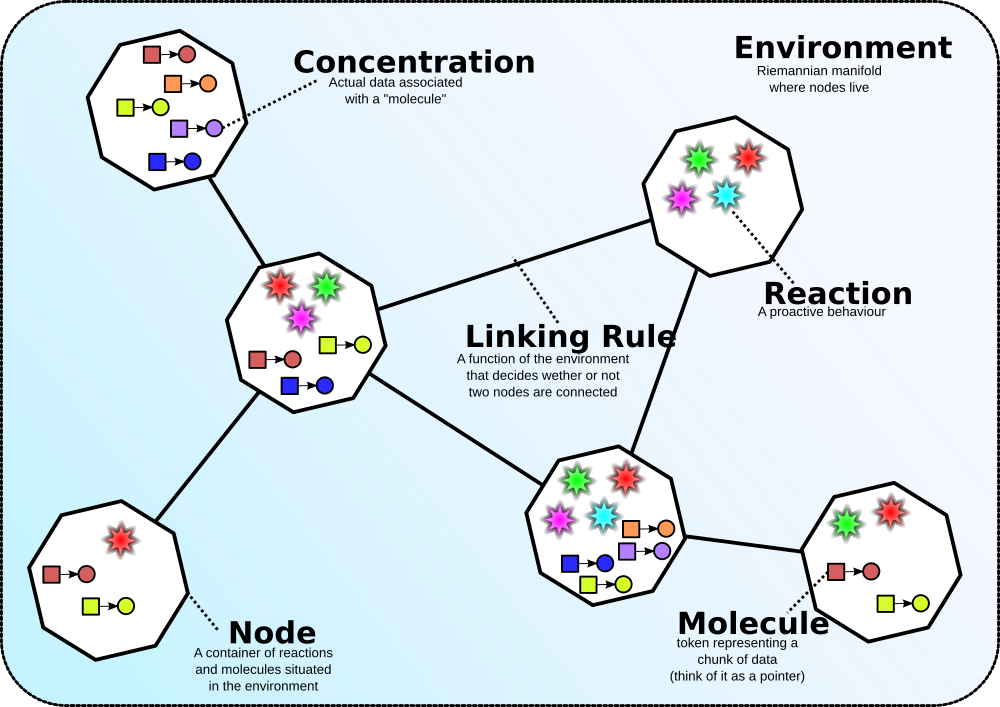
\includegraphics[width=12.5cm]{images/AlchemistModel.png} % inserisce una figura larga 12.5cm
% inserisce la legenda ed etichetta la figura con \label{fig:prima}
\caption[Illustrazione meta-modello di Alchemist]{Illustrazione meta-modello di Alchemist} \label{fig:alchemistModel}
\end{center}
\end{figure}

L'\textbf{\textit{Environment}} è l'astrazione dello spazio ed è anche l'entità più esterna che funge da contenitore per i nodi. Conosce la posizione di ogni nodo nello spazio ed è quindi in grado di fornire la distanza tra due di essi e ne permette inoltre lo spostamento.

\`E detta \textbf{\textit{Linking rule}} una funzione dello stato corrente dell'environment che associa ad ogni nodo un \textbf{\textit{Vicinato}}, il quale è un entità composta da un nodo centrale e da un set di nodi vicini.

Un \textbf{\textit{Nodo}} è un contenitore di molecole e reazioni che è posizionato all'interno di un environment.

La \textbf{\textit{Molecola}} è il nome di un dato, paragonabile a quello che rappresenta il nome di una variabile per i linguaggi imperativi.
Il valore da associare ad una molecola è detto \textbf{\textit{Concentrazione}}.

%crea l'ambiente figura;
\begin{figure}[h] % [h] sta per here, cioè la figura va qui
\begin{center} % centra nel mezzo della pagina la figura
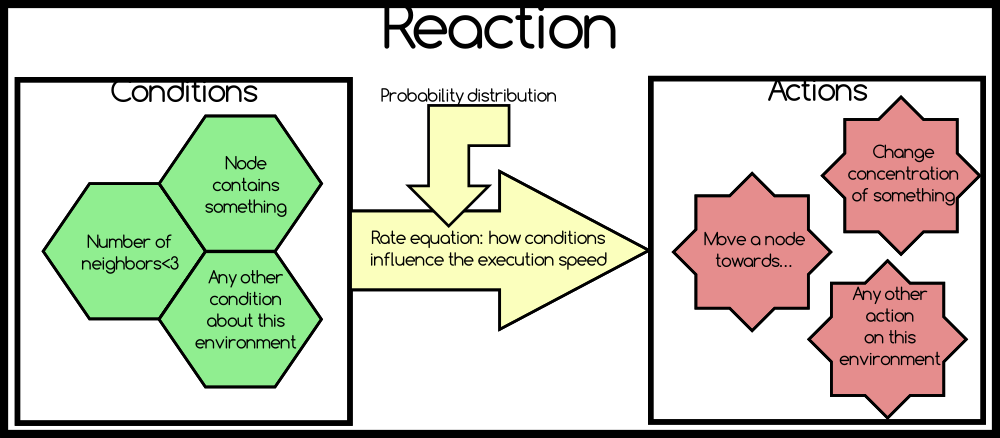
\includegraphics[width=14cm]{images/AlchemistReaction.png} % inserisce una figura larga 12.5cm
% inserisce la legenda ed etichetta la figura con \label{fig:prima}
\caption[Illustrazione modello reazione di Alchemist]{Illustrazione modello reazione di Alchemist} \label{fig:alchemistReaction}
\end{center}
\end{figure}

Una \textbf{\textit{Reazione}} è un qualsiasi evento che può cambiare lo stato dell'environment ed è definita tramite una distribuzione temporale, una lista di condizioni e una o più azioni.
\\La frequenza con cui avvengono dipende da:
\begin{itemize}
\item un parametro statico di frequenza;
\item il valore di ogni condizione;
\item un'equazione di frequenza che combina il parametro statico e il valore delle condizioni restituendo la frequenza istantanea;
\item una distribuzione temporale.
\end{itemize}
Ogni nodo contiene un set di reazioni che può essere anche vuoto.

Per comprendere meglio il meccanismo di una reazione si può osservare la figura \ref{fig:alchemistReaction}.

Una \textbf{\textit{Condizione}} è una funzione che prende come input l'environment corrente e restituisce come output un booleano e un numero. Se la condizione non si verifica, le azioni associate a quella reazione non saranno eseguite. In relazione a parametri di configurazione e alla distribuzione temporale, una condizione potrebbe influire sulla velocità della reazione.

La \textbf{\textit{Distribuzione temporale}} indica il numero di eventi, in un dato intervallo di tempo, generati da Alchemist e che innescano la verifica delle condizioni che possono portare alla potenziale esecuzione delle azioni.

Un'\textbf{\textit{Azione}} è la definizione di una serie di operazioni che modellano un cambiamento nel nodo o nell'environment.

In Alchemist un'incarnazione è un'istanza concreta del meta-modello appena descritta e che implementa una serie di componenti base come: la definizione di una molecola e del tipo di dati della concentrazione, un set di condizioni, le azioni e le reazioni. Incarnazioni diverse possono modellare universi completamente differenti.

%TODO \subsection{Esempi (?)}


%----------------------------
\section{LINDA}
LINDA è un modello di coordinazione e comunicazione tra diversi processi paralleli che operano su oggetti immagazzinati e recuperati dalla memoria associativa, virtuale, condivisa. Nel modello diverse primitive operano su una sequenza ordinata di oggetti, le `tuple', che vengono aggiunte ad un linguaggio sequenziale e una memoria associativa logica globale, detta spazio di tuple, nel quale i processi immagazzinano e recuperano le tuple.

Il modello LINDA originale definisce quattro operazioni consentite sulle tuple e lo spazio di tuple:
\begin{itemize}
\item \textit{in}: legge una tupla e la consuma dallo spazio di tuple
\item \textit{rd}: legge una tupla senza consumarla dallo spazio di tuple
\item \textit{out}: inserisce una tupla nello spazio di tuple
\item \textit{eval}: crea un processo per valutare le tuple e lo inserisce nello spazio di tuple.
\end{itemize}

LINDA è un modello di coordinazione utilizzato per definire altri modelli e tecnologie di coordinazione, dove gli agenti distribuiti interagiscono e si coordinano tramite scambio di messaggi utilizzando spazi di informazione condivisa e sfruttando la comunicazione generativa.

Di seguito è descritta un'estensione del modello appena descritto chiamata Spatial Tuples dove le informazioni base assumono una posizione e un'estensione nello spazio fisico.

\subsection{Spatial Tuples}
Spatial Tuples è un estensione del modello base di tuple per i sistemi distribuiti multi-agente, dove
\begin{itemize}
\item le tuple sono posizionate nel mondo fisico e si possono muovere;
\item il comportamento delle primitive di coordinamento può dipendere dalle proprietà spaziali del coordinamento degli agenti;
\item lo spazio di tuple può essere concepito come un livello virtuale che aumenta la realtà fisica.
\end{itemize}
Spatial Tuples supporta esplicitamente la consapevolezza dello spazio e la coordinazione basata sullo spazio dell'agente in scenari di calcolo pervasivo.

Questo modello può risultare molto utile in scenari dove gli utenti si spostano all'interno di un ambiente fisico aumentato e devono coordinarsi con altri utenti, che siano persone o agenti.

\subsubsection{Modello e linguaggio}
Spatial Tuples si occupa prima di tutto di tuple spaziali. Una tupla spaziale è una tupla associata ad un'informazione spaziale. Le informazioni spaziali possono essere, ad esempio, GPS, amministrative, organizzative: in ogni caso la tupla viene associata a qualche luogo o regione dello spazio fisico.
\\
Una tupla spaziale decora lo spazio fisico e può funzionare come meccanismo base per aumentare la realtà con informazioni di ogni sorta. Una volta che la tupla è associata ad una regione o posizione, le sue informazioni possono essere pensate come proprietà attribuite a quella porzione di spazio fisico. Accedendo alle tuple con i meccanismi di Spatial Tuples, l'informazione può essere osservata da qualsiasi agente che si occupa dello spazio fisico specifico in modo tale da comportarsi di conseguenza.
\\
Inoltre, una tupla può essere associata anche ad un componente situato. In questo caso, se il componente cambia la sua posizione nel tempo, finchè non viene rimossa, anche la tupla si sposterà con esso.

In Spatial Tuples viene introdotto un linguaggio di descrizione dello spazio per specificare le informazioni spaziali che decorano le tuple. Questo linguaggio è ortogonale al linguaggio di comunicazione e ha lo scopo di fornire l'ontologia di base che definisce i concetti spaziali.

\subsubsection{Primitive spaziali}
Gli operatori base di Spatial Tuples sono: $out(t), rd(tt), in(tt)$ dove $t$ è la tupla e $tt$ è un template di tupla. Il funzionamento delle primitive è il seguente:
\begin{itemize}
\item $out$, permette di associare la tupla ad una regione o posizione;
\item $rd$, cerca le tuple che corrispondono al template e ne ritorna una copia;
\item $in$, come $rd$, cerca le tuple che corrispondo al template ma poi ne restituisce una consumandola dalla sorgente.
\end{itemize}
Le primitive $rd$ e $out$ sono dette `getter' e, in Spatial Tuples, sono:
\begin{itemize}
\item sospensive, se non ci sono tuple che fanno match con il template l'operazione è bloccata finchè non viene trovata una tupla
\item non deterministiche, se vi sono più tuple che fanno match con il template una è scelta in modo non deterministico.
\end{itemize}


\chapter{AgentSpeak in tuProlog}\label{chap:agentspeak-2p}
Nel capitolo precedente è stato descritto lo stato attuale di lavori correlati che utilizzano il modello ad agenti BDI per costruirne altri più complessi ed espressivi o implementano linguaggi basati sugli agenti. Inoltre, è stato mostrato lo stato dell'arte delle tecnologie che sono state utilizzate.

In questo lavoro di tesi si è voluto definire un nuovo linguaggio che fosse \textit{`platform indipendent'}, ovvero indipendente dall'ambiente sul quale viene utilizzato: è stato definito al pari di una libreria, senza nessun riferimento all'ambiente. Nei capitoli successivi verrà mostrato come, partendo dal linguaggio, è stata colmata la distanza con l'ambiente scelto.

\section{Definizione linguaggio}\label{sctn:definizioneLinguaggio}
Essendo tuProlog un interprete che opera su piattaforme differenti, si è voluto utilizzarlo nella definizione del linguaggio per permettere di utilizzare quest'ultimo facilmente, potendo sfruttare la libreria tuProlog per colmare la distanza tra l'ambiente e il linguaggio.

Seguendo quella che è la struttura di AgentSpeak, è stato formalizzato questo linguaggio di programmazione ad agenti, e, di seguito, sono mostrate le definizioni.

\smallskip
% Definizione 1
\begin{defn}
Se $b$ è un simbolo di predicato e $t_1, \ldots, t_n$ sono termini, allora $belief(b(t_1, \ldots, t_n))$ è un atomo di belief.
Se $belief(b(t))$ e $belief(c(s))$ sono atomi di belief, allora $belief(b(t)) \land belief(c(s))$ e $\neg belief(b(t))$ sono beliefs.
Un atomo di belief oppure la sua negazione sono riferiti al letterale del belief. Un atomo di belief base sarà chiamato \textit{belief base}.
\end{defn}

\smallskip
% Definizione 2
\begin{defn}\label{defn:goals}
Se $g$ è un simbolo di predicato e $t_1, \ldots, t_n$ sono termini, allora $achievement(g(t_1, \ldots, t_n))$ e $test(g(t_1, \ldots, t_n))$ sono \textit{goals}.
\end{defn}

\smallskip
% Definizione 3
\begin{defn}\label{defn:triggeringEvents}
Se $b(t)$ è un atomo di belief e $g(t)$ un goal, allora $onAddBelief(b(t))$, $onRemoveBelief(b(t))$, $onReceivedMessage(b(t))$, $onResponseMessage(b(t))$,  $con\-cur\-rent(achieve\-ment(g(t)))$, $concurrent(test(g(t)))$ sono \textit{eventi di attivazione}.
\end{defn}

\smallskip
% Definizione 4
\begin{defn}
Se $a$ è un simbolo di azione e $t_1, \ldots, t_n$ sono termini del primo ordine, allora $a(t_1, \ldots, t_n)$ è un'azione.
\end{defn}

\smallskip
% Definizione 5
\begin{defn}
Se $e$ è un \textit{evento di attivazione}, $b_1, \ldots, b_m$ sono belief o guardie e $h_1, \ldots, h_n$ sono goals o azioni, allora $\text{\leftArrow}(e, [b_1, \ldots, b_m], [h_1, \ldots, h_n])$ è un piano.
Il contesto è definito da $[b_1, \ldots, b_m]$, mentre il corpo da $[h_1, \ldots, h_n]$. Il contesto vuoto o il corpo vuoto sono definiti entrambi da $[true]$.
\end{defn}

\smallskip
% Definizione 6
\begin{defn}
Un \textit{agente} è formato da $\langle B,P,I,A,S_O,S_I \rangle$, dove $B$ è una `belief base', $P$ è un set di piani, $I$ è un set di intenzioni, $A$ è un set di azioni. La funzione $S_O$ sceglie un piano dal set di quelli applicabili; la funzione $S_I$ sceglie l'intenzione da eseguire dal set $I$.
\end{defn}

\smallskip
% Definizione 7
\begin{defn}\label{defn:intenzione}
Ogni intenzione ha al suo interno uno stack di piani parzialmente istanziati, ovvero dove alcune delle variabili sono state istanziate. Un'intenzione è definita come $intention(i, [p_1, \ldots, p_n])$, dove $i$ è l'identificativo univoco dell'intenzione e $[p_1, \ldots,p_n]$ è lo stack formata da azioni, belief o goal: $p_1$ è la coda e $p_n$ è la testa.
\end{defn}

\smallskip
% Definizione 8
\begin{defn}
Dato un evento $\epsilon$ ed un piano $p = \text{\leftArrow}(e, [b_1, \ldots, b_m], [h_1, \ldots, h_n])$, allora $p$ è rilevante per l'evento $\epsilon$ se e solo se esiste un unificatore $\sigma$ tale per cui $d\sigma = e\sigma$. $\sigma$ è detto \textit{unificatore rilevante} per $\epsilon$.
\end{defn}

\smallskip
% Definizione 9
\begin{defn}
Un piano $p$ è definito da $\text{\leftArrow}(e, [b_1, \ldots, b_m], [h_1, \ldots, h_n])$ è un \textit{piano applicabile} rispetto ad un evento $\epsilon$ se e solo se esite un identificatore rilevante $\sigma$ per $\epsilon$ e esiste una sostituzione $\theta$ tale che $\forall (b_1, \ldots, b_m) \sigma\theta$ è una conseguenza logica di $B$.
%La composizione $\sigma\theta$ è riferita all'\textit{unificatore applicabile} per l'evento $\epsilon$ e $\theta$ è riferita alla sostituzione della corretta risposta.
\end{defn}

\smallskip
% Definizione 11
\begin{defn}
Sia $S_O(O_\epsilon) = p$, dove $O_\epsilon$ è il set dei piani applicabili per l'evento $\epsilon$ e $p$ è $\text{\leftArrow}(e, [b_1, \ldots, b_m], [h_1, \ldots, h_n])$. Il piano $p$ è destinato all'evento $\epsilon$ se e solo se esiste un \textit{unificatore applicabile} $\sigma$ per cui $[i_1 \ddagger (\text{\leftArrow}(e, [b_1, \ldots, b_m], [h_1, \ldots, h_n])) \sigma] \in I$.
\end{defn}

\smallskip
% Definizione 13
\begin{defn}
Sia $S_I(I) = i$, dove $i$ è $[p_1 \ddagger \ldots \ddagger \text{\leftArrow}(e, [b_1, \ldots, b_m], [h_1, \ldots, h_n])]$. L'intenzione $i$ si dice che è eseguita se e solo se $h_1$ è eseguito.
\end{defn}

%\bigskip
%a-a-a-a-a-a-a-a-a-a-a-a-a-
%\smallskip
%% Definizione 14
%\begin{defn}
%Sia $S_I(I) = i$, dove $i$ è $[p_1 \ddagger \ldots \ddagger `\leftarrow'(e, [b_1, \ldots, b_m], [h_1, h_2, \ldots, h_n])]$. L'intenzione $i$ si dice che è eseguita se e solo se esiste una sostituzione $\theta$ tale che $\forall h_1 \theta$ è una conseguenza logica di B e $i$ è rimpiazzato da $[p_1 \ddagger \ldots \ddagger `\leftarrow'(e, [b_1, \ldots, b_m] \theta, [h_2 \theta, \ldots, h_n \theta])]$.
%\end{defn}
%
%\smallskip
%% Definizione 15
%\begin{defn}
%Sia $S_I(I) = i$, dove $i$ è $[p_1 \ddagger \ldots \ddagger f : c_1 \land \ldots \land c_y \leftarrow a(t); h_2; \ldots; h_n]$. L'intenzione $i$ si dice che è eseguita se e solo se $a(t) \in A$, e $i$ è rimpiazzato da $[p_1 \ddagger \ldots \ddagger f : c_1 \land \ldots \land c_y \leftarrow h_2; \ldots; h_n]$.
%\end{defn}
%
%\smallskip
%% Definizione 16
%\begin{defn}
%Sia $S_I(I) = i$, dove $i$ è $[p_1 \ddagger \ldots \ddagger p_{z-1} \ddagger g(t) : c_1 \land \ldots \land c_y \leftarrow true]$, dove $p_{z-1}$ è $e : b_1 \land \ldots \land b_x \leftarrow !g(s); h_2; \ldots; h_n$. L'intenzione $i$ si dice che è eseguita  se e solo se esiste una sostituzione $\theta$ tale che $g(t)\theta = g(s)\theta$ e $i$ è rimpiazzato da $[p_1 \ddagger \ldots \ddagger p_{z-1} \ddagger (e : b_1 \land \ldots \land b_x)\theta \leftarrow (h_2; \ldots; h_n) \theta]$.
%\end{defn}
%
%\bigskip
%a-a-a-a-a-a-a-a-a-a-a-a-a-

\section{API del linguaggio}
Il linguaggio appena definito è ciò che è messo a disposizione del programmatore dell'agente per descrivere il suo comportamento. Oltre questo, sono state definite altre sintassi che permettano al programmatore di gestire ogni evento o situazione per l'agente.
Qui di seguito sono citate regole, variabili e fatti del linguaggio:
\begin{itemize}
\item $init \impliedBy \ldots$
\item $self(A).$
\item $agent$
\item $node$
\item $addBelief(B).$
\item $removeBelief(B).$
\item $\text{\leftArrow}(onAddBelief(B), [b_1, \ldots, b_m], [h_1, \ldots, h_n]).$
\item $\text{\leftArrow}(onRemoveBelief(B), [b_1, \ldots, b_m], [h_1, \ldots, h_n]).$
\item $\text{\leftArrow}(onReceivedMessage(S,M), [b_1, \ldots, b_m], [h_1, \ldots, h_n]).$
\item $\text{\leftArrow}(achievement(T), [b_1, \ldots, b_m], [h_1, \ldots, h_n]).$
\item $\text{\leftArrow}(test(T), [b_1, \ldots, b_m], [h_1, \ldots, h_n]).$
\item $\text{\leftArrow}(concurrent(T), [b_1, \ldots, b_m], [h_1, \ldots, h_n]).$
\item $belief(position(X,Y)).$
\item $belief(distance(A, ND, OD)).$ oppure $belief(distance(A, ND)).$
\end{itemize}

Di seguito vengono analizzate ed esposte.
Per ogni regola è lasciata l'implementazione del corpo al programmatore dell'agente.

\paragraph*{}
La regola `$init$' è messa a disposizione per permettere di effettuare una configurazione iniziale dell'agente. Infatti, questa regola verrà invocata solo ed esclusivamente la prima volta che viene attivato l'agente, al posto del ciclo di ragionamento. In questo modo il programmatore dell'agente è in grado di far eseguire all'agente una serie di operazioni iniziali per impostare ad esempio la `belief base' dell'agente.

\paragraph*{}
Il fatto `$self(A)$' permette all'agente di recuperare il suo nome. In questo modo il nome dell'agente può essere recuperato anche all'interno della teoria tuProlog.

\paragraph*{}
I due letterali `$agent$' e `$node$' sono due variabili di tuProlog alle quali sono collegati gli oggetti dell'agente e del nodo, implementati nell'ambiente su cui si è scelto di utilizzare il linguaggio. Se costruiti correttamente, dalla teoria dell'agente sarà possibile richiamare metodi implementati nella classe corrispondente. La variabile `$agent$' fa riferimento all'oggetto dell'agente stesso, mentre `$node$' si riferisce all'oggetto che rappresenta lo spazio sul quale l'agente è inserito. In questo modo possono essere gestite le azioni interne ed esterne dell'agente.

\paragraph*{}
Le regole `$addBelief(B)$' e `$removeBelief(B)$' sono utilizzabili per aggiungere o rimuovere elementi dalla `belief base'. Il loro utilizzo scatena un evento che va ad invocare `$onAddBelief(B)$', `$onRemoveBelief(B)$'. Più precisamente `$onAddBelief(B)$' viene invocato quando viene aggiunto un belief, mentre `$onRemoveBelief(B)$' è chiamato in seguito alla rimozione di un belief dalla `belief base'. In entrambi i casi la variabile $B$ corrisponde al belief inserito o rimosso.

Diversamente, quando viene letto un messaggio ricevuto da un altro agente (o anche da se stesso), è invocato `$onReceivedMessage(S, M)$', dove $S$ rappresenta il mittente e $M$ il contenuto del messaggio, che consente all'agente di reagire quando viene letto un messaggio tra quelli presenti nella sua coda di ingresso.

\paragraph*{}
Come visto precedentemente nella Definizione \ref{defn:goals}, i letterali `$achievement$', `$test$' sono utilizzati per impostare dei goal nell'agente. Ciò che viene scatenato è l'inserimento della serie di operazioni definita dal goal in testa allo stack dell'intenzione.
In combinazione, i due letterali appena citati possono essere usati in combinazione con `$concurrent$', mostrato nella Definizione \ref{defn:triggeringEvents}, che permette di inserire le operazioni definite nel goal in una nuova intenzione. In questo modo, la nuova intenzione può essere eseguita in modo concorrente o parallelo rispetto a quella `padre'.

\paragraph*{}
Per rendere disponibile al programmatore dell'agente varie possibilità per accedere a informazioni quali la posizione dell'agente e la distanza degli altri agenti rispetto alla propria posizione, sono utilizzati due belief che saranno aggiornati direttamente dall'ambiente sul quale viene utilizzato il linguaggio. La posizione dell'agente viene aggiornata una volta per ogni ciclo di ragionamento e, al termine, sono modificati anche i valori dei belief appena citati.

Per quanto riguarda la posizione dell'agente, potrà essere invocato `$be\-lief(po\-si\-tion(X, Y))$' dove $X$ è la coordinata relative alle ascisse o longitudine e $Y$ è la coordinata relativa alle ordinate o latitudine.

La distanza da altri agenti può essere molto utile per far scegliere all'agente di effettuare o meno una certa azione. Se nella lista del vicinato entra un nuovo agente viene inserito il belief `$belief(distance(A, ND))$', dove $A$ è il nome dell'agente nel vicinato e $ND$ è la distanza che li separa. Se, invece, un agente era già nella lista del vicinato e vi rimane, allora viene inserito il belief `$belief(distance(A, ND, OD))$', dove $A$ è il nome dell'agente nel vicinato, $ND$ è la nuova distanza che li separa e $OD$ è la distanza che li divideva precedentemente.

\subsection{Gestione intenzioni}
Le intenzioni sono la modalità con cui l'agente opera le sue azioni. Come descritto in precedenza, nel ciclo di ragionamento alla sezione \ref{ssctn:cicloRagionamentoAgentSpeak}, l'agente esegue una serie di passi che portano all'esecuzione di un'azione.
Qui di seguito è descritto come avviene il ciclo di ragionamento utilizzando questo linguaggio. La spiegazione terrà conto solamente degli aspetti relativi alla parte tuProlog e quindi sarà incompleta fino al raggiungimento della sezione \ref{sctn:interpreteLinguaggio}. Le funzioni di selezione per i piani applicabili e le intenzioni non sono trattate in questa parte, poichè sono relative all'implementazione dell'interprete.

L'agente lato tuProlog definisce il suo comportamento tramite una serie di regole e fatti che gli permettono di reagire ad eventi sia esterni che interni. Una percezione dell'ambiente può essere scatenata ad esempio da uno spostamento o una modifica della `belief base': quando questo avviene l'ambiente sul quale è utilizzato il linguaggio invoca una delle regole che, se implementata correttamente nella teoria dell'agente, consente all'agente di reagire all'evento. Un altro tipo di input che può ricevere l'agente è la ricezione di un messaggio. In tuProlog l'agente può reagire alla lettura del contenuto del messaggio poichè l'implementazione e la gestione delle code e la selezione dei messaggi viene fatta dall'interprete.

La frequenza dell'esecuzione del ciclo di ragionamento dipende dall'ambiente sul quale viene utilizzato il linguaggio. All'interno del ciclo, una volta selezionato il piano applicabile per l'evento avvenuto, l'interprete invoca delle regole per ottenere la lista delle operazioni presenti nel corpo del piano (o regola) per poterle inserire nell'intenzione. Le regole per recuperare la lista eseguono per ogni elemento del corpo una lettura e un inserimento all'interno di una lista, la quale poi viene restituita.

La creazione dell'intenzione viene fatta dall'interprete ma salvata come fatto nella teoria dell'agente. Come descritto nella definizione \ref{defn:intenzione}, l'intenzione $in\-ten\-tion(id,[op_1, \ldots, op_n])$ è composta da un identificativo univoco $id$ e da una lista di operazioni $[op_1, \ldots, op_n]$. All'interno della teoria dell'agente possono essere presenti più intenzioni contemporaneamente ma ad ogni ciclo di ragionamento solo una verrà selezionata per l'esecuzione.
Come detto precedentemente, anche la selezione dell'intenzione è gestita dall'interprete ma lato tuProlog ne viene gestita l'esecuzione. Infatti, l'interprete si limita a invocare la regola $execute(I)$ all'interno della quale viene gestita l'esecuzione della prima operazione sullo stack dell'intenzione con identificativo $I$, ovvero quella che è stata precedentemente selezionata.

La regola $execute$ si occupa di recuperare l'intenzione riferita all'identificativo passato e quindi prendere la testa dello stack delle operazioni. Quest'ultima viene valutata ed in base alla sua natura vengono eseguite azioni diverse:
\begin{itemize}
\item le azioni vengono eseguite direttamente;
\item i goal vengono recuperati lo stack di operazioni collegate viene successivamente aggiunto in testa all'intenzione di cui faceva parte il goal;
\item i goal espressi all'interno di $concurrent$ creano una nuova intenzione che potrà essere eseguita in parallelo rispetto a quella da cui ha avuto origine la chiamata al goal.
\end{itemize}


\subsection{Estensione Spatial Tuples}
Il linguaggio appena descritto è stato esteso per permettere di utilizzare il modello Spatial Tuples. Sono state quindi inserite le seguenti regole:
\begin{itemize}
\item $writeTuple(T).$
\item $readTuple(TT).$
\item $takeTuple(TT).$
\item $onResponseMessage(M) \impliedBy \ldots$
\end{itemize}
Le regole dell'elenco sono tutte riferite all'inserimento, all'interno del linguaggio, del modello di coordinazione LINDA e più precisamente del modello Spatial Tuples.
Con questa estensione, viene data la possibilità agli agenti di poter inserire e recuperare informazioni posizionate nello spazio. Le regole messe a disposizione mappano le primitive dei modelli che vogliono implementare `\textit{in}', `\textit{rd}', `\textit{out}' rispettivamente in `$writeTuple(T)$', `$readTuple(TT)$', `$takeTuple(TT)$' dove $T$ è la tupla da inserire e $TT$ è il template da ricercare.

Utilizzando `$writeTuple(T)$' il programmatore è in grado di inserire informazioni posizionate nello spazio degli agenti e con le quali gli stessi agenti possono interagire. Per leggere le informazioni si possono utilizzare due diverse modalità: `$readTuple(TT)$' e `$takeTuple(TT)$'. Nel primo caso viene utilizzato il template passato per confrontarlo con le tuple nell'intorno dell'agente e se ci sono risultati che combaciano con il template allora uno di questi viene restituito. Per quanto riguarda invece `$takeTuple(TT)$', si comporta ugualmente per quanto riguarda la ricerca della tupla con il template ma poi, una volta trovati i risultati ne sceglie uno e prima di restituirlo lo elimina dallo spazio di tuple in cui era presente.
%
Entrambe le modalità che recuperano le informazioni, ovvero $readTuple(TT)$ e $takeTuple(TT)$, seguono la semantica standard dei modelli basati su tuple, e quindi sono:
\begin{itemize}
\item sospensive: se non ci sono tuple che si abbinano al template l'operazione è bloccata finchè non viene trovata una tupla;
\item non deterministiche: se ci sono più tuple che si abbinano al template una è scelta in modo non deterministico.
\end{itemize}
Per dare la possibilità di gestire la risposta e gestire la tupla restituita è stata introdotta `$onResponseMessage(M)$' che viene invocata ogni qualvolta che una tupla viene restituita dallo spazio di tuple. Il contenuto $M$ è la tupla incapsulata in un belief in modo che si possano gestire tuple provenienti da diversi spazi di tuple e con contenuti differenti.

\section{Esempi linguaggio}
In questa sezione verranno mostrate alcuni casi d'uso del linguaggio appena descritto. Nello specifico verrà mostrato un primo scenario dove sono stati configurati gli agenti per realizzare un semplice scambio di messaggi (o Ping Pong). Nel secondo esempio, invece, viene illustrato come poter utilizzare l'estensione Spatial Tuples supportata dal linguaggio.

\subsubsection{Ping Pong}
In questo primo esempio è presentato il problema del Ping Pong. In questo esempio sono definiti due agenti, Ping e Pong, ognuno dei quali risponde ad un messaggio ricevuto. L'agente Ping, alla ricezione del messaggio `\textit{pong}' da parte dell'agente Pong risponderà con un messaggio `\textit{ping}'. Viceversa, l'agente Pong, alla ricezione del messaggio `\textit{ping}' da parte dell'agente Ping risponderà con un messaggio `\textit{pong}'.

Per far iniziare lo scambio di messaggi è stato utilizzato `init' per impostare all'interno di uno dei due agenti, nello specifico l'agente Ping, un'intenzione iniziale. In questo modo, al primo ciclo di ragionamento, l'agente eseguirà l'intenzione e invierà il primo messaggio.

\switchToProlog{}
\begin{lstlisting}[float,firstnumber=1,label={lst:PingAgent},caption={Agente Ping}]
init :-
    agent <- generateNextRandom returns ID,
    asserta(intention(ID,[iSend('pong_agent','ping')])),
    agent <- insertIntention(ID).

'<-'(onReceivedMessage(S,pong),[true],[iSend(S, ping)]).
\end{lstlisting}

In entrambe le teorie dei due agenti è stata richiamata `$iSend(S, M)$', dove $S$ è il destinatario e $M$ è il messaggio, che è un'azione interna dichiarata e gestita nell'ambiente sul quale è utilizzato il linguaggio. Nel Codice sorgente \ref{lst:PingAgent} viene inviato all'agente Pong il messaggio `ping', mentre nel Codice sorgente \ref{lst:PongAgent} il messaggio inviato all'agente Ping è `pong'.

\switchToProlog{}
\begin{lstlisting}[float,firstnumber=1,label={lst:PongAgent},caption={Agente Pong}]
init :-
    true.

'<-'(onReceivedMessage(S,ping),[true],[iSend(S, pong)]).
\end{lstlisting}

\subsubsection{Message passing through Spatial Tuples}
In questo esempio viene mostrato come possono essere utilizzate le primitive del modello Spatial Tuples incorporate nel linguaggio descritto in precedenza. Nello specifico viene mostrato come tre agenti (Alice, Bob e Carl) comunicano tra loro inserendo messaggi negli spazi di tuple a loro vicini, usandoli come `lavagna'.
L'agente Alice nel suo ciclo di configurazione, esegue due scritture sulla `lavagna' (spazio di tuple) inserendo messaggi per Bob e Carl e successivamente effettua altre due richieste allo spazio di tuple richiedendo due messaggi a lei destinati senza conoscerne il contenuto. Una volta ricevuti i messaggi non fa niente.

\switchToProlog{}
\begin{lstlisting}[float,firstnumber=1,label={lst:Alice},caption={Alice}]
init :-
  writeTuple(bb,msg(bob,hello)),
  writeTuple(bb,msg(carl,hello)),
  takeTuple(bb,msg(alice,X)),
  takeTuple(bb,msg(alice,X)).

'<-'(onResponseMessage(msg(X,Y)),[true],[true]).
\end{lstlisting}

L'agente Bob, nel suo ciclo di configurazione, effettua una richiesta allo spazio di tuple per ricevere messaggi a lui destinati. Inoltre, nella sua teoria, è definito un comportamento in caso di ricezione del messaggio: manda ad Alice lo stesso messaggio che ha ricevuto.

\switchToProlog{}
\begin{lstlisting}[float,firstnumber=1,label={lst:Bob},caption={Bob}]
init :-
  takeTuple(bb,msg(bob,X)).

'<-'(onResponseMessage(msg(bob,X)),
		[true],[writeTuple(bb,msg(alice,X))]).
\end{lstlisting}

L'agente Carl esegue lo stesso comportamento di Bob.

\switchToProlog{}
\begin{lstlisting}[float,firstnumber=1,label={lst:Carl},caption={Carl}]
init :-
  takeTuple(bb,msg(carl,X)).

'<-'(onResponseMessage(msg(carl,X)),
		[true],[writeTuple(bb,msg(alice,X))]).
\end{lstlisting}


\chapter{AgentSpeak in tuProlog su Alchemist}\label{chap:agentspeak-2p-alchemist}
In questo capitolo verrà esposta la parte di implementazione mancante nel capitolo precedente. Più precisamente è descritto come è stato scelto di implementare il modello ad agenti su Alchemist, fornendo un'analisi del mapping, e di come è stato utilizzato il linguaggio per definire l'interprete, scendendo nel dettaglio di come è stata realizzata la gestione delle intenzioni, lo spostamento dell'agente e l'estensione Spatial Tuples. Ulteriori dettagli relativi all'implementazione verranno analizzati nel capitolo successivo.

La scelta della piattaforma è ricaduta su Alchemist poichè fornisce un meta-modello molto adattabile a vari ambiti applicativi e una struttura di simulazione già consolidata ed efficace.

Come detto in precedenza è possibile realizzare implementazioni del modello ad agenti utilizzando il linguaggio definito in questo lavoro di tesi anche sfruttando altre piattaforme che consentono di lavorare con la libreria tuProlog.

\section{Mapping modelli}\label{sctn:mapping}
In precedenza sono stati descritti il modello ad agenti e il meta-modello di Alchemist. Ora, dopo aver definito il linguaggio, per procedere all'implementazione è necessario capire quale sia il migliore modo, in termini di performance e espressività, per unire i due modelli.
In questa fase si vuole quindi pensare come realizzare sul meta-modello fornito da Alchemist il modello ad agenti cercando eventuali incongruenze o opportunità per massimizzare il risultato.

Si è partiti analizzando le entità del meta-modello e per ognuna è stato posto l'interrogativo sul fatto che potesse rappresentare l'agente.
Fin da subito sono state ritenute inadatte l'Environment e la Molecola: il primo perchè è esso stesso lo spazio e non avrebbe potuto rappresentare l'ambiente degli agenti; la Molecola perchè fornisce un livello di dettaglio troppo elevato e non ha una struttura che consente di contenere lo stato dell'agente.

Le entità rimaste da analizzare sono quindi il Nodo e la Reazione, la quale contiene Condizioni e Azioni.

Mappando il Nodo come agente ne deriva che l'Environment corrisponderà allo spazio degli agenti mentre, all'interno dell'agente, le Molecole e le relative Concentrazioni potranno essere utilizzate per gestire la `belief base' e le Reazioni saranno riferite ai piani, utilizzando le Condizioni come clausola per scatenare le Azioni. Questo tipo di mapping consente di realizzare simulazioni di sistemi non complessi, in cui agenti allo stesso livello operano e comunicano tra loro.

Posizionando l'agente nella Reazione, quindi più internamente rispetto al precedente mapping, il Nodo diventerà un contenitore di agenti e l'Environment lo spazio nel quale si muovono i nodi. Ogni agente avrà il riferimento ad una Condizione e ad una Azione: quest'ultima conterrà il ciclo di ragionamento dell'agente mentre la Condizione ne determinerà la clausola di esecuzione (che in questo caso è impostata per essere sempre vera e scatenare periodicamente l'azione). Utilizzando questa seconda ipotesi sarà possibile realizzare simulazioni di sistemi complessi, nei quali dei nodi, che potrebbero essere dispositivi mobili (ad esempio cellulari), si muovo nello spazio ed ognuno al suo interno contiene un gruppo di agenti che possono interagire sia internamente che esternamente.

Dopo aver analizzato le due possibili alternative presentate, è stato scelto il mapping in cui l'agente è posizionato nella Reazione poichè permette una maggiore espressività e un'apertura verso più scenari applicativi.

\section{Descrizione interprete linguaggio}\label{sctn:interpreteLinguaggio}
Una volta scelto il mapping si è iniziato lo sviluppo dell'interprete del linguaggio sul meta-simulatore al fine di creare una `incarnazione', ovvero il nome con cui sono chiamate le implementazioni dei modelli in Alchemist.

Alchemist è un meta-simulatore che, proprio per la sua natura di simulatore, ha un meccanismo di generazione degli eventi e fornisce quindi la possibilità di gestire lo scheduling dei cicli di ragionamento degli agenti. Più precisamente, in Alchemist è possibile definire una distribuzione temporale per ogni reazione, la quale, nell'incarnazione che si vuole realizzare e secondo il mapping scelto, corrisponde ad un agente. È quindi possibile decidere quante volte viene programmata l'iterazione del ciclo di ragionamento di ogni singolo agente. La scelta fatta per gestire la distribuzione temporale è ricaduta sull'utilizzo di un pettine di Dirac che è una distribuzione periodica degli eventi costruita da una somma di delta di Dirac, la quale è una funzione generalizzata che dipende da un parametro reale utilizzata per rappresentare dei picchi, le iterazioni del ciclo di ragionamento.

Si è pensato come organizzare le invocazioni delle regole base, definite dal linguaggio, per migliorare l'usabilità dell'interprete. È stato deciso di creare una classe astratta all'interno della quale implementare le funzionalità principali dell'agente, le quali saranno utili al programmatore dell'agente nella realizzazione delle classi specifiche degli agenti poichè sarà sufficiente richiamare queste funzioni se non sono necessari comportamenti specifici.

\subsection{Implementazione del linguaggio}\label{sctn:ImplementazioneLinguaggio}
Il primo passo è stato quello di definire la libreria dell'agente, ovvero l'implementazione delle chiamate messe a disposizione del programmatore dell'agente. Sono state quindi definite, utilizzando le funzionalità base di tuProlog, le regole per aggiungere o rimuovere un belief, per eseguire un'intenzione.
% e per recuperare la lista di operazioni dal corpo di un piano, quest'ultima solo per uso interno.
La definizione di queste regole è stata necessaria per permettere la gestione dei cicli di ragionamento, cioè per consentire ad Alchemist di riprendere il controllo alla fine del ciclo di ragionamento di ogni agente evitando così che un agente possa eseguire le sue operazioni entrando in un loop infinito.
Ad esempio la definizione per l'aggiunta e la rimozione dei belief è quella mostrata nel Codice sorgente \ref{lst:ImplementazioneRegoleModificaBeliefBase} nella quale sono eseguite due operazioni: la prima riguarda l'effettiva modifica della `belief base' con il belief passato, mentre la seconda inserisce un belief fittizio recuperato dall'interprete per permettere di innescare l'evento di modifica del relativo belief al prossimo ciclo di ragionamento.

\switchToProlog{}
\begin{lstlisting}[float,firstnumber=1,label={lst:ImplementazioneRegoleModificaBeliefBase},caption={Implementazione regole modifica della `belief base'}]
addBelief(B) :-
  assertz(belief(B)),
  assertz(added_belief(B)).

removeBelief(B) :-
  retract(belief(B)),
  assertz(removed_belief(B)).
\end{lstlisting}

Una modalità analoga è stata utilizzata per gestire anche altri eventi, sempre per poter separare l'invocazione della regola dall'attivazione dell'evento. Gli eventi in questione sono quelli relativi alla realizzazione dell'estensione Spatial Tuples e che sono stati implementati come mostrato nel Codice sorgente \ref{lst:ImplementazioneRegoleSpatialTuples}. In questo caso sono aggiunti dei fatti il cui contenuto è la tupla o il template da utilizzare nella richiesta verso lo spazio di tuple.

\switchToProlog{}
\begin{lstlisting}[float,firstnumber=1,label={lst:ImplementazioneRegoleSpatialTuples},caption={Implementazione regole estensione Spatial Tuples}]
writeTuple(T) :-
  assertz(write(T)).

readTuple(T) :-
  assertz(read(T)).

takeTuple(T) :-
  assertz(take(T)).
\end{lstlisting}

\subsection{Invocazione regole ed esecuzione intenzioni}\label{sctn:InvocazioneEsecuzioneIntenzioni}
Terminata la definizione delle regole per la gestione degli eventi è stata aggiunta la libreria \texttt{`alice.tuprolog’} dalla quale è stato importato all'interno della classe dell'agente il motore tuProlog per la realizzazione delle invocazioni verso la teoria dell'agente.
Le API di tuProlog permettono a Java di sfruttare il motore Prolog: gli oggetti istanziati che rappresentano entità Prolog (termini, atomi, liste, variabili, numeri e anche teorie e librerie) che possono essere utilizzate per effettuare interrogazioni e ottenere il risultato lato Java \cite{2p-alpnews2013}.
Ogni istanza dell'agente ha un motore tuProlog al cui interno è caricata la libreria che implementa il nuovo linguaggio e una teoria specifica scritta dal programmatore dell'agente che descrive il comportamento dell'agente.

L'agente nel meta-modello è riferito all'entità Reazione ma nell'implementazione il ciclo di ragionamento dell'agente, ovvero il cuore, risiederà nell'Azione: la classe che definisce l'agente implementerà l'interfaccia relativa a tale entità.

Per fare un'invocazione, da Alchemist, di fatti o regole definiti nella teoria dell'agente vengono utilizzate alcune funzionalità messe a disposizione dalla libreria \texttt{'alice.tuprolog'} che sono descritte qui di seguito.

La prima cosa da fare è costruire il template del fatto o della regola che si vuole ottenere.
Gli oggetti standard di Prolog, quali numeri interi e float, sono mappati nella classe Term \cite{tuPrologLight-weight}. Questa classe è la radice della gerarchia, fornendo sia la gestione diretta dei tipi primitivi sia l'interfaccia di base per tutti i termini. \cite{tuPrologLight-weight}.
Sfruttando le classi della libreria tuProlog si possono utilizzare due modi: creazione del termine o composizione della struttura del termine. Nel primo caso viene invocata la funzione statica $Term.createTerm(t)$ dove il parametro passato è una stringa che descrive la struttura del template. Diversamente, la composizione della struttura del termine utilizza la classe Struct. Per creare un oggetto di questo tipo si devono definire almeno un funtore, di tipo stringa, e un termine, che può essere un numero, una variabile o un'altra struttura. In questo modo la creazione del termine del template risulta molto più efficiente.

Terminata la costruzione del template è il momento di effettuare l'interrogazione all'interno della teoria dell'agente. Per fare questo viene utilizzata la funzione $solve(term)$ definita all'interno del motore tuProlog e che restituisce un oggetto dal quale è possibile ricavare i risultati dell'interrogazione, come ad esempio:
\begin{itemize}
\item controllare se la richiesta è andata a successo;% (funzione $isSuccess$);
\item recuperare il valore di una singola variabile inserita nel template;% (funzione $getTerm$);
\item ottenere la soluzione del template, ovvero dove tutte le variabili utilizzate sono sostituite con il valore del fatto o della regola ricavato;% (funzione $getSolution$);
\item verificare se ci fossero altre possibili alternative che corrispondono al template utilizzato;% (funzione $hasOpenAlternatives$);
\end{itemize}

Per quanto riguarda invece l'esecuzione dell'intenzione sono state definite una serie di regole che, utilizzando l'identificativo, recuperano l'intenzione e ne prelevano la lista di operazioni collegate. Se la lista è vuota allora l'intenzione viene rimossa. Altrimenti si preleva l'operazione in testa, la quale viene eseguita e restituisce una lista con eventuali operazioni da eseguire scaturite dal suo processamento (ed esempio se l'azione è un goal). La nuova lista di operazioni viene quindi aggiunta in testa alla lista delle operazioni già presenti nell'intenzione e poi quest'ultima viene aggiornata. Quanto appena descritto è mostrato nel Codice sorgente \ref{lst:ImplementazioneRegoleInvocazioneEsecuzioneIntenzione}.

È inoltre necessario descrivere in che modo vengono selezionati i piani applicabili e le intenzioni per completare la descrizione degli step che sono effettuati.

Per quanto riguarda la selezione delle azioni internamente viene utilizzata la selezione del motore tuProlog che sfrutta l'ordinamento con cui sono definite le regole e i fatti nella teoria. Una volta selezionata l'azione viene eseguita.
Per quanto riguarda la selezione dei piani relativi agli eventi e ai goal, la selezione avviene utilizzando il contesto, ovvero la guardia, che permette di definire se un piano è applicabile a quella certa situazione.
Una volta selezionato il piano viene creata un'intenzione che è opportunamente inserita nella lista delle intenzioni.

Diversamente, per quanto riguarda l'intenzione da eseguire avviene la seguente gestione.
Nella teoria dell'agente sono salvate tutte le intenzioni mentre nell'interprete viene salvata una lista contenente solamente gli identificativi delle rispettive intenzioni presenti nella teoria. La tipologia di selezione è Round-Robin, ogni intenzione avrà lo stesso spazio di esecuzione delle altre. L'intenzione da eseguire viene presa dalla testa dello stack e una volta finita la sua esecuzione viene posizionata in coda: in questo modo si assicura che ogni intenzione possa essere eseguita.

\switchToProlog{}
\begin{lstlisting}[float, firstnumber=1,label={lst:ImplementazioneRegoleInvocazioneEsecuzioneIntenzione},caption={Implementazione regole per invocazione esecuzione di un'intenzione}]
execute(I) :-
    intention(I, []), !,
    agent <- removeCompletedIntention(I).

execute(I) :-
    retract(intention(I, [ACTION | STACK])),
    execute(I, ACTION, TOP), !,
    append(TOP, STACK, NEWSTACK),
    assertz(intention(I, NEWSTACK)).
\end{lstlisting}

\subsection{Gestione azioni}\label{sctn:GestioneAzioni}
L'esecuzione vera e propria dell'intenzione è gestita da altre regole che sono definite ciascuna per ogni tipologia: $achievement$, $test$, $concurrent$, azione interna e azione esterna; qui di seguito verrà descritto come sono state implementate ognuna di esse.

In caso l'azione da eseguire fosse un $achievement$ allora, una volta verificata la correttezza del contesto (detto anche guardia), il contenuto del corpo di quella regola (una serie di invocazioni a fatti o altre regole) verrà recuperato e restituito per essere aggiunto in testa allo stack dell'intenzione da cui è pervenuta l'invocazione di quell'azione. Lo stesso comportamento verrà tenuto per azioni di tipo $test$.

Diversamente, se si tratta dell'azione $concurrent$, sia che essa racchiuda $achieve\-ment$ o $test$, il suo obiettivo è quello di creare un intenzione concorrente a quella dalla quale è pervenuta l'invocazione dell'azione. Per fare questo, per prima cosa si ottiene la regola verificandone la correttezza del contesto e poi si recupera la sua lista di operazioni, che è contenuta nel corpo.
A questo punto viene generato un nuovo identificativo univoco per l'intenzione ed infine è creato il fatto dell'intenzione così formato: $intention(id, [op_1, \ldots, op_n])$, dove $id$ è l'identificativo generato e $[op_1, \ldots, op_n]$ la lista di operazioni contenute nel corpo della regola invocata.

Per quanto riguarda le azioni interne ed esterne, cioè che rispettivamente accadono nell'agente o nell'ambiente, il programmatore dell'interprete è in grado di definirne di nuove in base al contesto applicativo in cui si deve calare il linguaggio e l'interprete. Un esempio di definizione di un'azione interna è quello relativo all'azione per inviare dei messaggi. Per realizzarlo è stata definita la sintassi $iSend(S,M)$, dove $S$ è il mittente e $M$ messaggio. Quando un'azione interna o esterna viene richiamata per l'esecuzione deve essere verificata la sua esistenza prima che possa essere eseguita: per fare questo possono essere definiti dei fatti, come ad esempio $is\_internal(iSend(S,M))$, per essere utilizzati come template per la validazione della sintassi. Il controllo funziona come una guardia e, se ha successo, l'operazione interna può essere eseguita richiamando un'apposita funzione implementata all'interno della classe dell'agente invocabile tramite l'oggetto $agent$ presente nella teoria. Per comodità si potrebbe implementare all'interno dell'agente un'unica funzione, ad esempio $executeInternalAction(action)$ che viene sempre richiamata per l'esecuzione di azioni interne e che, in base al parametro in ingresso, sceglie quale azione eseguire.
In modo analogo possono essere modellate le azioni esterne gestite dal nodo, che rappresenta lo spazio dell'agente. Infatti, la scelta di riferire all'interno della teoria dell'agente anche l'oggetto del nodo permette di poter implementare azioni per l'agente che abbiano effetto nell'ambiente.

\subsection{Spostamento del nodo}\label{sctn:SpostamentoNodo}
Precedentemente nella sezione \ref{sctn:mapping} si è trattato dello spazio, ovvero dell'ambiente in cui gli agenti si muovono. Con il mapping scelto per l'implementazione del meta-modello sono presenti due livelli di spazio: uno internamente al nodo, il contenitore degli agenti, e l'altro che è l'ambiente globale dove si possono muovere i nodi.
Il nodo quindi è visto non come un singolo agente ma come un gruppo di agenti che è in grado di muoversi nello spazio, che in base all'ambito applicativo può essere sia fisico che simulato. All'interno della classe del nodo sarà implementata la funzionalità per gestire il movimento.

Nell'implementazione che è stata effettuata si sono utilizzate due variabili, memorizzate come proprietà della classe, per la gestione dello spostamento: la direzione (espressa in radianti) e la velocità. Inoltre, è stato utilizzato un altro parametro, il tempo (tau) dell'ultimo aggiornamento della posizione, per poter calcolare l'esatta posizione finale del nodo trascorso un certo arco temporale. In questo modo, avendo possibilità di gestire tutti i parametri (direzione, velocità, tempo) è possibile calcolare lo spostamento del nodo in una qualsiasi posizione.

La funzione che calcola la nuova posizione del nodo è descritta nel Codice sorgente \ref{lst:ImplementazioneAggiornamentoPosizioneNodo}. Date la posizione attuale del nodo $(P_X,P_Y)$, la direzione in radianti $D$, la velocità del nodo $V$ e il tau (tempo della simulazione) $T_0$ dell'ultimo aggiornamento della posizione. Viene costruito un cerchio che ha come centro $(P_X,P_Y)$ e il cui raggio ha distanza uguale a $V * (T_1 - T_0)$, dove $T_1$ è il tempo corrente della simulazione. Sulla circonferenza appena creata viene individuata la prossima posizione del nodo calcolando il punto che corrisponde alla direzione $D$ attualmente memorizzata nel nodo.

\switchToJava{}{\small}
\begin{lstlisting}[float,firstnumber=1,label={lst:ImplementazioneAggiornamentoPosizioneNodo},caption={Implementazione aggiornamento posizione nodo}]
void changeNodePosition(Time t1) {
  Position currPos = this.getNodePosition();

  double radius = (t1.toDouble() - this.t0.toDouble()) * this.speed;

  double coordX = currPos.getCoordinate(0) + radius * Math.cos(this.radAngle);

  double coordY = currPos.getCoordinate(1) + radius * Math.sin(this.radAngle);

  this.environment.moveNodeToPosition(this, this.environment.makePosition(coordX, coordY));

  this.t0 = t1;
}
\end{lstlisting}

Per rispettare il fatto che il movimento sia una funzione basilare dell'implementazione ad agenti si è pensato a come realizzarlo. Richiamare la funzione appena descritta dentro ogni agente non è il modo migliore poichè potrebbe essere invocata più di una volta ed essere quindi aggiornata troppo frequentemente.

L'idea che è stata poi realizzata è quella di inserire all'interno di ogni nodo un agente che abbia come unico compito quello di innescare l'aggiornamento della posizione del nodo stesso e di comunicare la variazione a tutti gli altri agenti all'interno. Per fare ciò, il modo migliore è stato quello di inserire, durante la creazione del nodo, un agente al suo interno, il quale, come detto precedentemente, avrà il compito di innescare l'aggiornamento della posizione del nodo e successivamente di far partire l'adeguamento interno di ogni agente riguardo la sua posizione (che è quella del nodo) e la distanza rispetto a tutti gli altri agenti (sia residenti nello stesso nodo nei nodi del vicinato).

Questo agente che gestisce il movimento ha una distribuzione temporale uguale a 1, ovvero il suo ciclo di ragionamento viene eseguito 1 volta ogni `clock' dello scheduler. In questo modo, definendo opportunamente la distribuzione temporale degli altri agenti della simulazione si può ottenere il risultato come se l'aggiornamento della posizione provenisse da un componente esterno, ad esempio un apparato GPS, che periodicamente aggiorna la posizione.

\subsection{Implementazione Spatial Tuples}\label{sctn:ImplementazioneSpatialTuples}
La realizzazione lato Alchemist del modello Spatial Tuples è stata fatta sfruttando il lavoro già svolto precedentemente per gli agenti. Partendo dalla classe definita per gli agenti si è deciso di estenderla per creare una nuova classe con la quale sarà possibile creare implementazioni specifiche per gli spazi di tuple. Per implementare correttamente il modello Spatial Tuples e gestire opportunamente le sue primitive è necessario però sviluppare due parti: la prima riguarda l'implementazione della classe che descrive il modello per gli spazi di tuple, mentre la seconda è relativa alla definizione di funzioni nella classe dell'agente per poter gestire le invocazioni delle primitive del linguaggio.

Sfruttando l'ereditarietà, lo spazio di tuple è implementato come un agente, anche se con le sue precise caratteristiche. La classe degli spazi di tuple è stata implementata estendendo la classe dell'agente e poi sono state definite ulteriori proprietà, ovvero due liste: una per i messaggi in entrata e una per quelli in attesa, ovvero che sono stati analizzati ma non hanno trovato una corrispondenza.
Il resto delle proprietà utilizzate, come ad esempio il motore tuProlog, il nome dell'agente e la libreria, sono ereditate dal padre e lo stesso vale anche per il costruttore.

L'agente effettua verso lo spazio di tuple delle richieste, ognuna delle quali è composta da un termine (che può essere una tupla o un template), un identificativo dell'azione e l'oggetto dell'agente, al quale poi comunicare la risposta.
Per la gestione delle due code sono state implementate altrettante funzioni, una per ogni coda, e in base al tipo di azione inserita nella richiesta ricevuta ($in$, $rd$, $out$) viene invocato il metodo per eseguire quella primitiva. Le operazioni vanno a modificare la teoria dello spazio di tuple scrivendo, leggendo o rimuovendo fatti tramite il motore tuProlog.

L'implementazione dell'operazione $in$ viene sempre eseguita immediatamente, poichè non è un'operazione bloccante, e al termine richiama la funzione che sblocca eventuali richieste di $rd$ e $out$, controllando se nella lista delle richieste pendenti vi siano template che corrispondano alla tupla appena inserita.

Le operazioni $rd$ e $out$ sono gestite in modo simile tra loro, cambia solo la natura del termine che viene poi eseguito tramite il motore tuProlog: nel primo caso contiene solo il template di selezione, mentre nel secondo anche la sintassi per rimuovere la tupla.
In entrambe le situazioni, se il motore restituisce almeno una tupla, ne viene presa una ( implementativamente è stato scelto di restituire la prima trovata) e inviata tramite risposta diretta all'agente.

In questo modo si è implementato lo spazio di tuple in modo generico, consentendo la possibilità di creaere classi specifiche per implementare le funzioni mancanti o riscrivere quelle presenti in modo diverso.
Ora è necessario parlare della parte da definire nella classe dell'agente che consentirà a quest'ultimo di interagire con gli spazi di tuple.

Nella classe dell'agente rimane da realizzare la parte per inviare una richiesta allo spazio di tuple e per ricevere in risposta le tuple richieste: per fare questo si sono implementati due funzioni.

La prima funzione è quella che recupera i fatti `fittizi' a seguito dell'invocazione di una delle regole definite nel Codice sorgente \ref{lst:ImplementazioneRegoleSpatialTuples} e successivamente li utilizza per creare la richiesta. Nell'implementazione realizzata si sono voluti tenere due approcci diversi per la scrittura e per la lettura di tuple: nel primo caso è stato scelto di posizionare la tupla solo nello spazio di tuple più vicino, mentre nel secondo caso il template viene confrontato con tutti gli spazi di tuple nell'intorno dell'agente.
La possibilità di relazionarsi con uno o più spazi di tuple è fornita dal modo in cui è stato implementato il nodo poichè permette di recuperare la lista degli agenti presenti in ogni nodo del suo vicinato, includendo quindi anche gli spazi di tuple. La lista può essere opportunamente filtrata successivamente in base alle necessità. Questa parte sarà descritta più chiaramente nella sezione \ref{sctn:AgentsContainerNode}.

L'altra funzione da implementare, è quella che consente all'agente di ricevere il messaggio di ritorno dallo spazio di tuple quando viene trovata la tupla che corrisponde al template inviato nella richiesta. La funzione in questione verrà descritta nella sezione \ref{sctn:AbstractAgent}.


\chapter{Dettagli implementativi e di deploy}\label{chap:impl}
In questo capitolo sono descritti alcuni dettagli relativi all'implementazione dell'interprete che è stato realizzato in Alchemist. In particolare verrà descritta la gerarchia delle classi definite all'interno dell'incarnazione e successivamente le proprietà e le funzionalità di quelle principali: Incarnation (AgentIncarnation), Node (AgentsContainerNode), Action (AbstractAgent).

Successivamente sono descritti gli strumenti utilizzati per supportare lo sviluppo di questo progetto: Gradle per la gestione delle librerie all'interno di Alchemist, GitHub per la gestione del repository e del codice sorgente, Travis CI per il monitoraggio di eventuali anomalie prodotte.

Infine, è presente una panoramica relativa alla costruzione della configurazione di una simulazione in Alchemist. Vengono descritte le varie parole chiave che possono essere utilizzate per caratterizzare la simulazione e, al termine, viene fornito un esempio di una configurazione per la simulazione.

\section{Note implementative}
Dopo aver già descritto i tratti principali dell'interprete per il modello ad agenti implementato all'interno di Alchemist, in questa sezione sono mostrate alcune caratterizzazioni più specifiche di come è stata realizzata l'incarnazione, con un focus verso le principali entità del modello e sulla struttura delle classi .
Inoltre verrà fatta una descrizione degli strumenti di sviluppo utilizzati per l'elaborazione del progetto.

\subsection{Gerarchia delle classi}
Precedentemente in questo lavoro si è accennato alle classi dell'incarnazione utilizzate per realizzarla limitandosi però solamente ad alcune informazioni generiche. In questa sezione l'obiettivo è quello di descrivere in maniera più accurata le classi, il funzionamento e le loro gerarchie all'interno dell'implementazione dell'interprete che è stata realizzata.

L'immagine presente in Figura \ref{fig:UMLGerarchiaClassi} mostra lo schema UML delle classi realizzate.
%crea l'ambiente figura;
\begin{figure}%[ht] % [h] sta per here, cioè la figura va qui
%\begin{center} % centra nel mezzo della pagina la figura
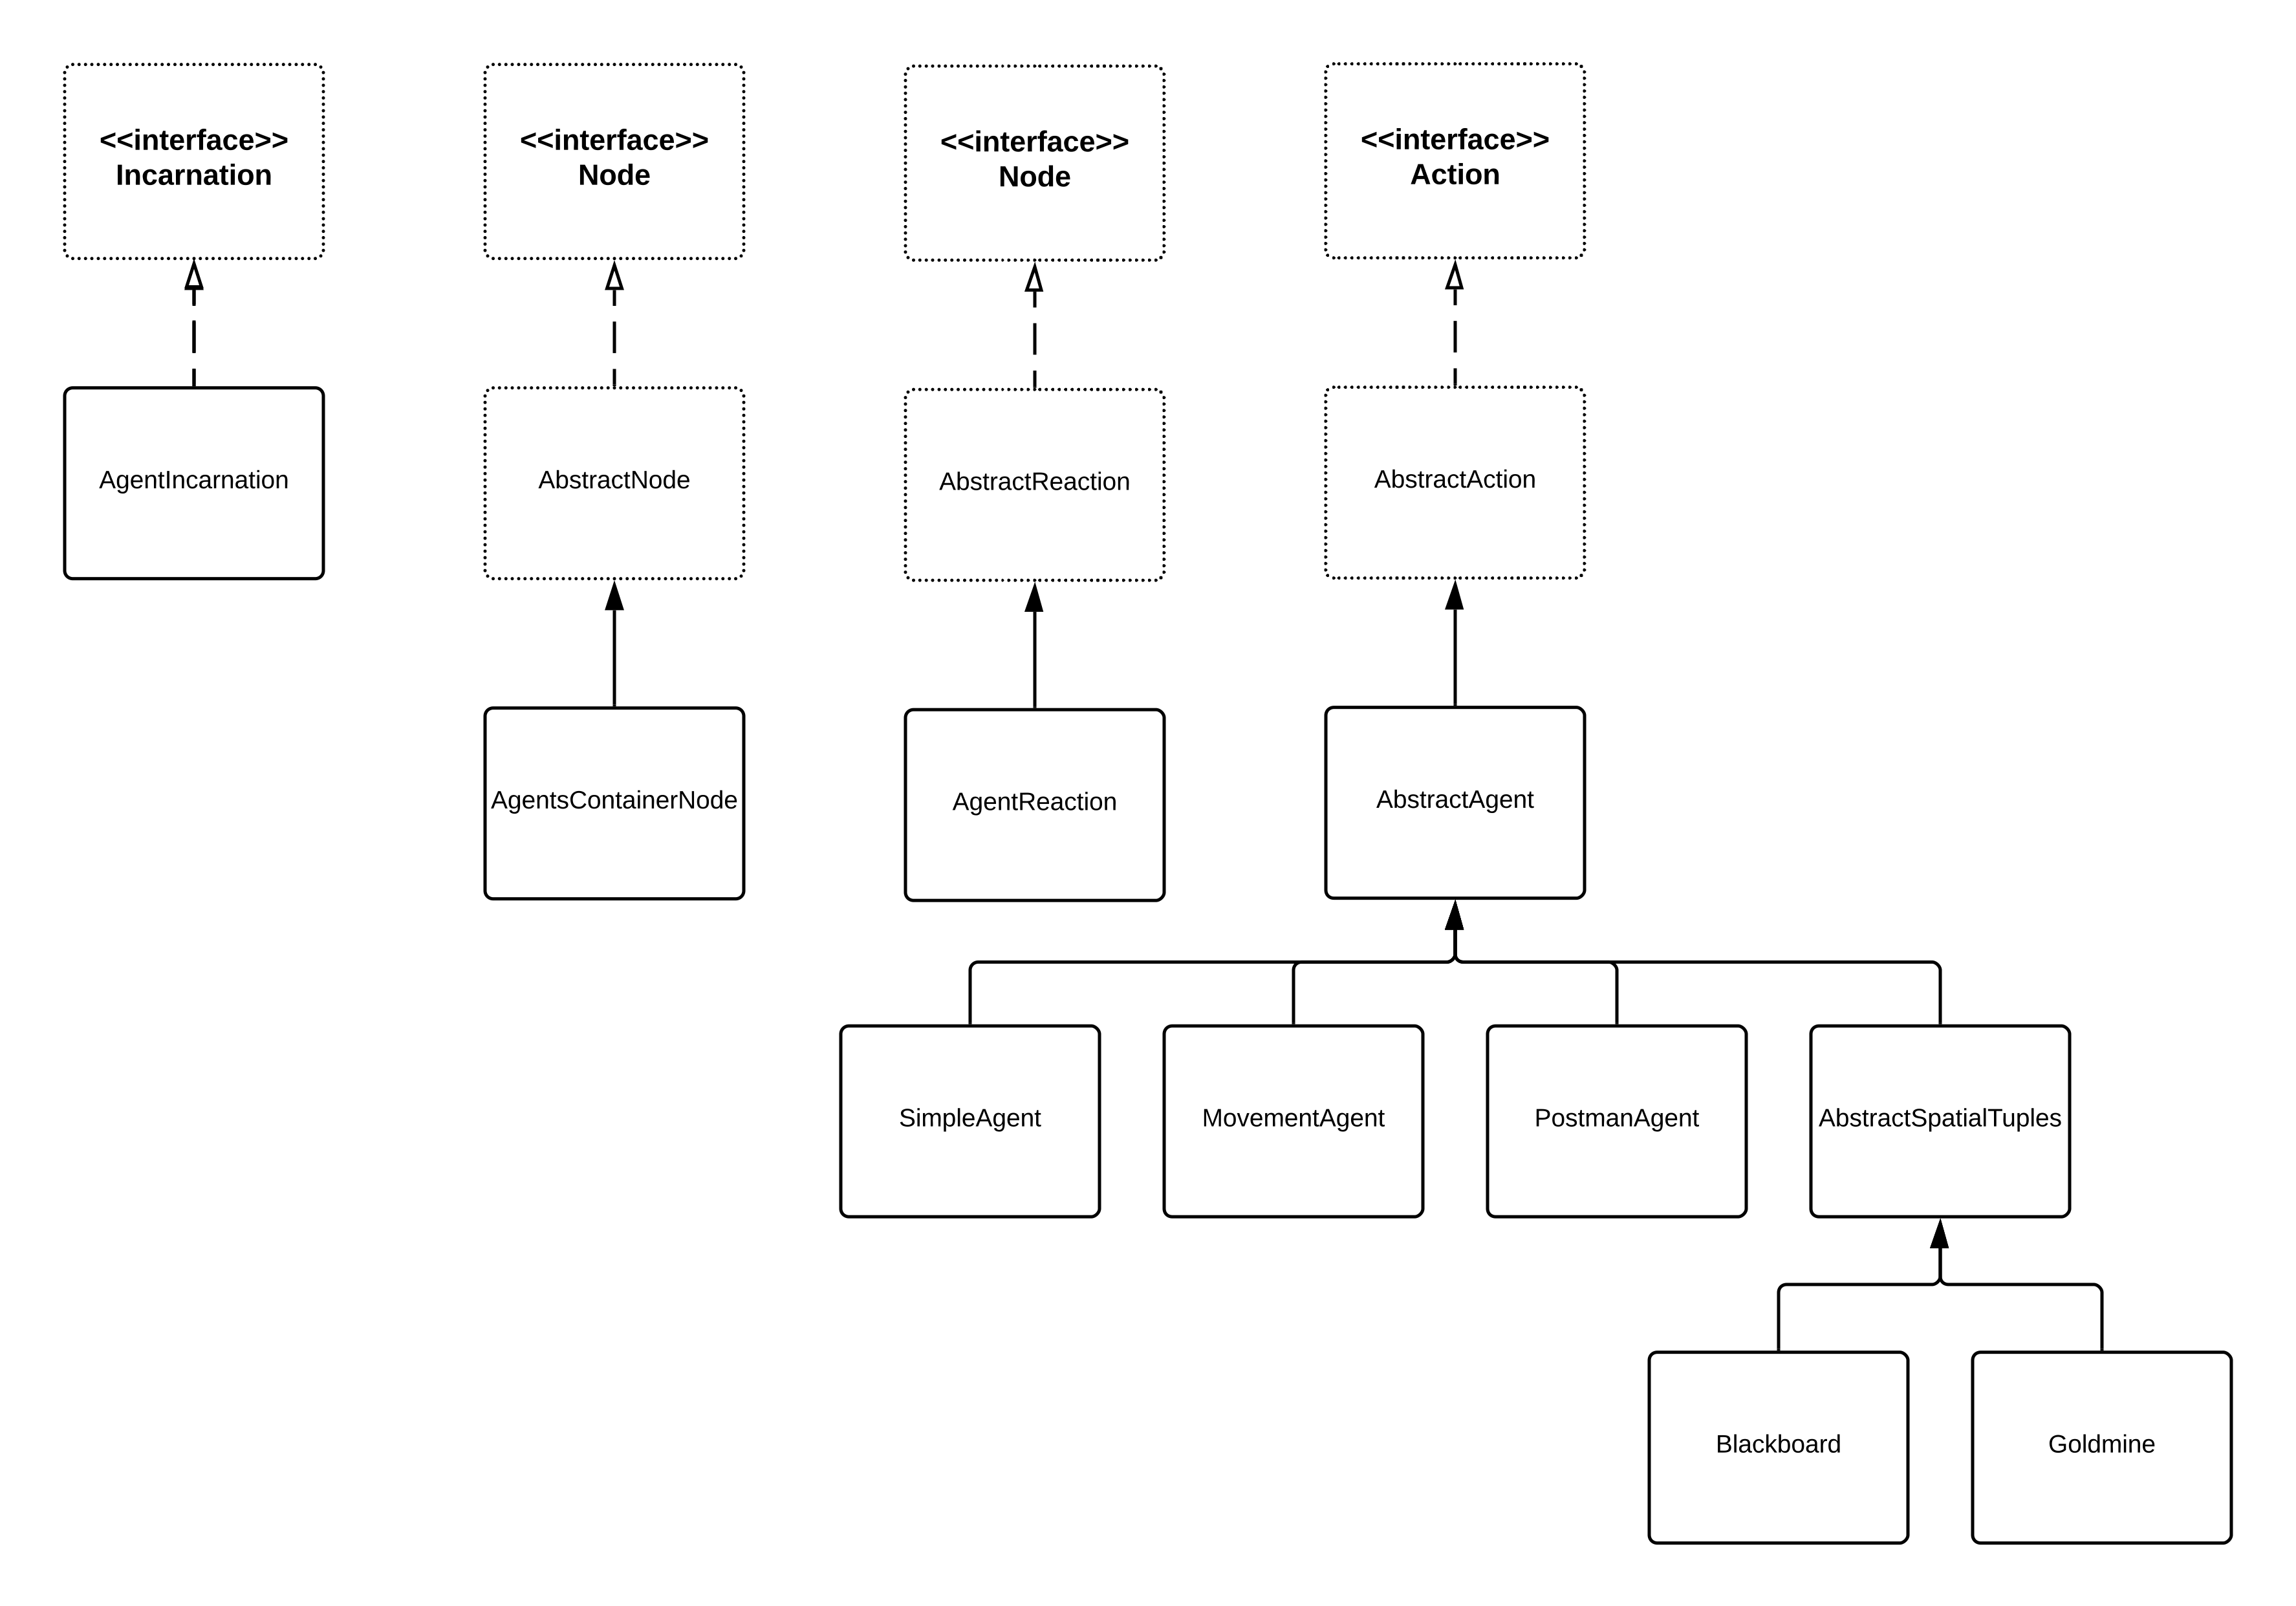
\includegraphics[width=15cm]{images/UML_agenti.png} % inserisce una figura larga 12.5cm
% inserisce la legenda ed etichetta la figura con \label{fig:prima}
\caption[Ricostruzione UML della gerarchia delle classi]{Ricostruzione UML della gerarchie delle classi} \label{fig:UMLGerarchiaClassi}
%\end{center}
\end{figure}

Lo schema rappresenta in modo informale la gerarchia di alcune classi e mostra la loro struttura ereditaria; quest'ultima comprende alcune classi o interfacce già implementate in Alchemist e pronte per essere utilizzate. I riquadri con il bordo tratteggiato distinguono le classi che non sono state definite per questa specifica incarnazione ma sono già presenti all'interno del simulatore: questo rende possibile utilizzare e lavorare con il simulatore in maniera più efficiente. Le restanti classi, rappresentate in riquadri con un bordo continuo, sono le classi implementate per realizzare, in questa specifica incarnazione di Alchemist, l'interprete per il nuovo linguaggio ad agenti.

Per quanto riguarda le frecce, quelle con la linea tratteggiata stanno ad indicare la relazione `implements', ovvero che una certa classe implementa l'interfaccia indicata, mentre quelle con il tratto continuo significano `extends', ovvero che una classe estende le proprietà e le funzionalità di quella da cui deriva.

Nello schema si può notare che la classe dell'incarnazione è stata realizzata partendo direttamente dall'implementazione dell'interfaccia: la struttura di questa classe verrà descritta nella sezione \ref{sctn:AgentIncarnation}.

Diversamente, per il Nodo e la Reazione si è scelto di estendere le rispettive classi astratte già presenti all'interno di Alchemist, le quali al loro interno implementano l'interfaccia di riferimento. La classe del nodo verrà spiegata più in dettaglio nella sezione \ref{sctn:AgentsContainerNode}, mentre per la reazione, che è l'entità individuata per rappresentare l'agente, è stata implementata la classe senza conferire particolare caratteristica poichè il core dell'agente è realizzato, come già accennato nella sezione \ref{sctn:InvocazioneEsecuzioneIntenzioni}, in un'entità contenuta al suo interno, ovvero l'Azione.

Come si può vedere dallo schema l'azione è l'entità che ha avuto il maggior numero di implementazioni. Per la realizzazione dell'Azione si è partiti descrivendo le funzionalità generiche dell'agente all'interno di una classe astratta per fornire un'esemplificazione e una base di partenza da poter utilizzare con poco sforzo o eventualmente ampliare per realizzare comportamenti specifici.
Ad esempio, per l'integrazione del modello SpatialTuples è stata estesa la classe base dell'agente per realizzare una nuova classe astratta (AbstractSpatialTuple) che, allo stesso modo della classe padre, offre la possibilità di utilizzare degli spazi di tuple avendo già una solida base di partenza. La classe dell'agente è descritta nella sezione \ref{sctn:AbstractAgent}.
Le altre classi implementate a partire dalla classe AbstractAgent sono implementazioni specifiche di agenti che sono state utilizzate per la realizzazione di simulazioni di scenari di test. Le classi che estendono AbstractSpatialTuple sono anch'esse realizzate come agenti ma incarnano il comportamento degli spazi di tuple.

\subsection{L'incarnazione}\label{sctn:AgentIncarnation}
Per realizzare la classe principale dell'incarnazione, e solo per questo caso, è stata implementata direttamente la corrispondente interfaccia, ovvero Incarnation.
Questa interfaccia definisce i metodi per poter implementare in maniera specifica ogni singola entità del meta-modello di Alchemist. All'interno della classe AgentIncarnation, che implementa appunto l'interfaccia Incarnation, sono state implementate le varie funzioni che, in fase di esecuzione, saranno opportunamente richiamate dal simulatore. Qui di seguito viene fornita una breve descrizione di come sono stati implementati i metodi definiti nell'interfaccia.

All'interno del metodo per la creazione di un oggetto dell'entità Molecola viene creata un'istanza della classe SimpleMolecule, implementazione già presente all'interno di Alchemist, che a partire da una stringa (utilizzata come identificativo) crea una corrispondente molecola.

Per quanto riguarda la Distribuzione Temporale, come accennato nella sezione \ref{sctn:SpostamentoNodo}, viene utilizzata la classe DiraComb, già implementata in Alchemist, che permette di creare eventi periodici ad una distanza temporale definita tramite un parametro.

Per creare il Nodo sono utilizzati i riferimenti all'Environment, che è utilizzato per gestire funzionalità come lo spostamento e il vicinato, e al RandomGenerator, il quale è impiegato per ottenere randomicità negli agenti. All'interno del metodo per la creazione di un Nodo è invocato il costruttore della classe AgentsContainerNode che ne fornisce un'istanza: l'oggetto creato è poi restituito all'applicazione per essere utilizzato durante la simulazione.

Per poterne gestire lo spostamento, come accennato nella sezione \ref{sctn:SpostamentoNodo}, all'interno di ogni nodo è stato inserito uno specifico agente incaricato di questo compito. L'operazione di inserimento avviene all'interno del metodo per la creazione del Nodo; dopo aver ottenuto un'istanza di AgentsContainerNode si crea una Reazione, che al suo interno conterrà l'azione per gestire il movimento, la quale è aggiunta al nodo prima di essere restituito.
%
Per creare questa Reazione, viene eseguito lo stesso procedimento descritto all'interno dell'apposito metodo definito all'interno della classe ma variando le funzioni invocate e la tipologia di alcuni oggetti istanziati.

Per creare una `normale' Reazione viene per prima cosa creata un'istanza della classe AgentReaction e poi invocati i metodi per creare le istanze di azioni e condizioni, passando gli opportuni parametri che specificano, tra gli altri, la classe dell'oggetto da istanziare. A questo punto, gli oggetti ottenuti dall'invocazione delle due funzioni, vengono inseriti all'interno dei rispettivi set della reazione, la quale viene infine ritornata.

Nel caso della reazione per lo spostamento, sono create sul momento le istanze degli oggetti che andranno a crearla e con il seguente ordine:
\begin{itemize}
\item[1.] TimeDistribution, tramite invocazione del metodo $createTimeDistribution$ implementato nella classe AgentIncarnation;
\item[2.] AgentReaction;
\item[3.] MovementAgent;
\item[4.] Condition, tramite invocazione del metodo $createCondition$ implementato nella classe AgentIncarnation.
\end{itemize}
%L'ordine è importante poichè la distribuzione è utilizzata all'interno della reazione, che a sua volta è utilizzata per creare l'azione e la condizione ad essa relativi.
Con la stessa modalità descritta appena sopra, le istanze di azione e condizione sono inserite all'interno di specifici set della reazione che, infine, viene inserita nel nodo. Questa è una reazione particolare poichè viene costruita `manualmente' (non tramite apposita funzione) e viene inserita `nativamente' nel nodo per comandare il suo movimento.
%
Inoltre, un passaggio che viene eseguito nella funzione di creazione della Reazione, è l'invocazione di un metodo, implementato nel nodo, il quale registra ogni nuovo agente all'interno di una struttura dati. Questo passaggio consente ad ogni nodo di mantenere traccia di tutti gli agenti presenti al suo interno e rende possibile recuperare il riferimento di ogni agente, anche esternamente rispetto al nodo a cui appartiene, in qualsiasi momento.
L'agente per lo spostamento non viene inserito nella struttura dati descritta e potrà essere individuato solamente recuperandolo dal nodo tramite le funzioni messe a disposizione da Alchemist.

La creazione della condizione è gestita in modo che questa risulti sempre vera e che quindi, secondo il meta-modello di Alchemist, vengano sempre scatenate le azioni collegate alla relazione a cui appartiene quella certa condizione. L'oggetto condizione che viene restituito dal metodo $createCondition$, invocato dall'interprete, è un'istanza della classe AbstractCondition che viene completata implementando la definizione del contesto (che impatta sulle performance della simulazione) e della condizione di validità (che come accennato poc'anzi è impostata per essere sempre vera).

Infine parliamo della creazione di oggetti dell'entità Azione. Per la creazione di queste istanze in base ad una valutazione del parametro ricevuto, che è stato passato dalla creazione della reazione, viene definita quale sia la classe dell'istanza da creare.
L'istanza dell'oggetto opportunamente inizializzata viene quindi ritornata per essere utilizzata all'interno di una reazione.
Al momento sono gestiti i casi per le seguenti classi:
\begin{itemize}
\item SimpleAgent
\item PostmanAgent
\item BlackboardAgent
\item GoldmineAgent
\end{itemize}


\subsection{Il contenitore degli agenti -- Nodo}\label{sctn:AgentsContainerNode}
Il nodo, nell'implementazione dell'interprete realizzata, è uno spazio (o contenitore di agenti) che gestisce i comportamenti dell'agente verso l'esterno, come ad esempio lo spostamento del nodo stesso e l'esecuzione di azioni esterne, ma implementa anche una serie di funzioni utili alla gestione della comunicazione tra agenti (recupero dell'elenco degli agenti nel vicinato, gestione dei messaggi fra agenti). Il nodo, come detto precedentemente, è definito tramite la classe AgentsContainerNode creata estendendo la classe astratta AbstractNode che a sua volta implementa l'interfaccia Node.

All'interno della classe sono definite le proprietà che contengono l'ambiente, il generatore random, i valori per gestire lo spostamento del nodo ed una struttura per il monitoraggio degli agenti presenti al suo interno.
Le istanze di Environment e RandomGenerator sono create all'interno del core di Alchemist e poi passate al costruttore della classe che le memorizza all'interno della classe. %, dopo averle registrate, inizializza inoltre la variabile che mantiene il tempo per dell'ultimo aggiornamento della posizione.
La struttura dati scelta è una mappa formata da una serie di coppie di valori composti da una chiave, che rappresenta il nome dell'agente, ed il valore, che è il riferimento stesso dell'agente. Attraverso questa struttura il nodo è in grado di recuperare il riferimento di ogni singolo agente presente al suo interno; questa implementazione, come vedremo di seguito, è stata molto utile per produrre nuove funzionalità specifiche implementate nel nodo.

Oltre alle proprietà, all'interno della classe sono presenti i metodi per la gestione della posizione, della mappa che monitora gli agenti e del vicinato calcolato in base a diversi criteri.

\`E quindi possibile impostare o recuperare i valori di direzione e velocità oppure ottenere la posizione stessa del nodo. Ovviamente è presente il metodo mostrato nel Codice sorgente \ref{lst:ImplementazioneAggiornamentoPosizioneNodo} che effettua il calcolo per ottenere le coordinate della nuova posizione del nodo.
Inoltre, è implementato il metodo $updateAgentsPosition()$ che innesca l'aggiornamento dei fatti, quali posizione e distanza dagli altri agenti, per ogni agente all'interno del nodo. Secondo l'implementazione attuale, questo metodo viene invocato solamente dall'agente `Movement', inserito alla creazione del nodo, che, nel suo ciclo di ragionamento, ha come unico compito quello di invocare questo metodo per scatenare l'aggiornamento. Gli agenti quindi verranno aggiornati quando lo scheduler di Alchemist farà eseguire il ciclo di ragionamento dell'agente `Movement'.

Per la gestione della mappa, utilizzata per il monitoraggio degli agenti, sono presenti due metodi: uno per effettuare l'inserimento, invocato come descritto nella sezione \ref{sctn:AgentIncarnation} durante la creazione di istanze dell'entità Reazione, e uno per ottenere la struttura completa.

Il concetto di vicinato viene gestito da Alchemist attraverso la funzione di linking-rule, che utilizza il parametro `network-model' se opportunamente impostato in fase di configurazione della simulazione.
Lato implementativo, è sufficiente richiedere all'Environment di fornire tutti i nodi presenti nel vicinato con i quali è poi possibile effettuare altre operazioni come, ad esempio, ottenere la distanza tra i vari nodi e recuperare gli agenti presenti in ogni nodo, utilizzando l'apposita mappa.

Lo stesso meccanismo è utilizzato per recuperare e operare negli spazi di tuple, definiti utilizzando l'estensione SpatialTuples. In questo caso, non è stato sufficiente il solo recupero di tutti i nodi ma sono stati applicati i filtri per ottenere solo gli agenti la cui istanza derivi da AbstractSpatialTuple.
Secondo la scelta implementativa effettuata, è necessario specificare due insiemi differenti per le diverse primitive invocabili sullo spazio di tuple: la scrittura è fatta su un solo spazio di tuple, ovvero quello più vicino, mentre la lettura su tutti quelli del vicinato.
Il secondo caso è il più immediato poichè si recupera l'elenco di tutti gli agenti presenti nei nodi del vicinato e si verifica solamente che l'istanza dell'agente sia un'implementazione della classe astratta AbstractSpatialTuple. Ogni agente che corrisponde a questa condizione viene aggiunto ad una lista, la quale è poi ritornata come output.

Diversamente, per quanto riguarda la scrittura, serve individuare lo spazio di tuple più vicino, recuperandolo tramite la mappa di agenti del nodo che lo contiene. Utilizzando l'ambiente, vengono confrontate le distanze di tutti i nodi rispetto a quello attuale e, si recupera quello più vicino che contiene almeno un'agente che sia istanza della classe astratta AbstractSpatialTuple. Di quel nodo viene selezionato il primo agente trovato che corrisponde ai canoni poichè verosimilmente, in base alle scelte implementative, in ogni nodo vi è un solo spazio di tuple.

Un altro metodo implementato all'interno della classe AgentsContainerNode è $postman()$ per la gestione dei messaggi, in modo simile a quanto realizzato per lo spostamento del nodo. Un'agente dedicato, chiamato `Postman' invoca un metodo che recupera tutti i messaggi in uscita da tutti gli agenti dell'ambiente e li consegna al corretto destinatario. Maggiori dettagli di questa funzionalità sono descritti nella sezione \ref{sctn:DettaglioImplementazioni}.

Inoltre, sempre all'interno della classe del nodo, è stato scelto di implementare il metodo, invocabile dalla teoria dell'agente, per la gestione delle azioni esterne.
La scelta di implementare questa funzionalità all'interno del nodo è dovuta alla sua posizione nell'ambiente rispetto al modello e al mapping scelto poichè è lo snodo in cui si ha la possibilità di interagire sia con l'ambiente che con gli agenti di altri nodi. Si è quindi implementato il metodo $executeExternalAction(String action)$ all'interno del quale, in base all'azione ricevuta come parametro, viene selezionata una serie di operazioni che portano al raggiungimento di quella certa azione. Come invocare funzionalità implementate in Alchemist dalla teoria è mostrato nella sezione \ref{sctn:DettaglioImplementazioni}.

\subsection{L'agente -- Azione}\label{sctn:AbstractAgent}
L'agente è il punto centrale dell'incarnazione che è stata realizzata, dal quale sono partiti tutti i ragionamenti per il design dell'interprete e la mappatura del modello ad agenti sul meta-modello di Alchemist.

Come già detto precedentemente, l'agente è stato associato alla Reazione che però non è essa stessa l'entità operativa, ovvero quella che viene eseguita periodicamente, ma solo il contenitore. L'entità Azione è la parte che il simulatore richiama attivamente per l'esecuzione se le condizioni, anch'esse contenute nella Reazione, validano le proprie clausole.

Per la realizzazione della classe dell'agente si è scelto, anche in questo caso, di partire da un'implementazione già fornita da Alchemist, ovvero dalla classe astratta AbstractAction.

La scelta successiva è stata quella relativa al design della classe da implementare. Dopo un'accurata analisi è stato scelto di realizzare, invece che un'implementazione definitiva, una classe astratta che descrive le proprietà base dell'agente e ne implementa le funzionalità principali (inizializzazione dell'agente e gestione di messaggi, di `belief base', di intenzioni e di operazioni negli spazi di tuple), lasciando comunque al programmatore la scelta della caratterizzazione dell'agente. La scelta di creare una classe astratta è dovuto al fatto di non voler dare nessuna implementazione del ciclo di ragionamento ma fornire implementazioni dei comportamenti e azioni basilari che lo compongono: in questo modo è possibile facilmente definire nuovi comportamenti o creare agenti partendo da quelli già realizzati.

Non sono quindi implementati i metodi $execute()$, $cloneAction(node, reaction)$, definiti dall'interfaccia Action, dalla cui implementazione è caratterizzato il comportamento dell'agente. In particolare, il metodo $execute()$, che è quello che rappresenta il ciclo di ragionamento, è invocato periodicamente dal core di Alchemist (questo perchè le Condizioni collegate alla stessa Reazione sono impostate per essere sempre vere) per lo svolgimento delle azioni.

All'interno della classe sono definite le seguenti proprietà: due code per i messaggi (una per quelli in entrata e una per quelli in uscita), il motore tuProlog, lo stack contenente gli identificativi delle intenzioni presenti nella teoria, riferimenti alla reazione e al generatore random.

La classe astratta dell'agente gestisce, inoltre, la teoria dell'agente e sfrutta il motore tuProlog importato tramite l'apposita libreria `alice.tuprolog'. Attraverso questo componente è possibile caricare una teoria ed effettuare interrogazioni della stessa permettendo all'agente di operare raccogliendo i risultati per creare intenzioni o inserire nuove informazioni.

Per inizializzare un agente sono state definite una serie di operazioni posizionate poi all'interno dei metodi $initializeAgent()$ e $initReasoing()$.
Questi due metodi hanno come obiettivo quello di inizializzare l'agente: il primo lo fa dalla parte dell'interprete mentre il secondo configura l'inizializzazione dello stato iniziale dell'agente.
Entrambi, per la corretta configurazione dell'agente in relazione all'implementazione attuale, dovrebbero essere richiamati all'interno del ciclo di ragionamento solamente una volta, ovvero alla prima iterazione, per completare la configurazione dell'agente iniziata nel costruttore.

All'interno del metodo $initializeAgent()$ viene caricata nel motore tuProlog la libreria dell'agente, quella descritta nel capitolo precedente e che implementa il linguaggio definito in questo lavoro di tesi, a cui segue il caricamento della teoria specifica che definisce il comportamento di un certo agente. Successivamente, sempre all'interno dello stesso metodo, viene eseguita la registrazione di oggetti Java all'interno della teoria (questa azione verrà descritta in dettaglio nella sezione \ref{sctn:DettaglioImplementazioni}) e l'inserimento all'interno della teoria dell'agente del fatto $self(nome\_agente)$ che completa la procedura di inizializzazione da parte dell'interprete.

Nel metodo $initReasoning()$ viene eseguita una sola operazione, ovvero l'invocazione della regola $init$ che permette al programmatore dell'agente di eseguire una configurazione dello stato iniziale dell'agente.
Al termine di queste due operazioni si può considerare l'agente completamente inizializzato e pronto per reagire a tutti i possibili eventi per cui è stato programmato.

All'interno dell'agente, utilizzando il generatore random, è definita una proprietà per la gestione della casualità che è un'istanza della classe LevyDistribution, definita nel package `org.apache.commons.math3.distribution', la quale permette di creare una distribuzione random a partire da un randomizzatore. Questa distribuzione è messa a disposizione insieme al randomizzatore per fornire all'agente casualità da utilizzare nelle sue operazioni. Ad esempio può essere utilizzata per generare valori per la velocità e la direzione del nodo che contiene l'agente.

Per quanto riguarda lo scambio di messaggi, l'agente implementa i metodi per inserire e recuperare i messaggi dalle sue code che sono richiamati opportunamente dall'agente `Postman' descritto nella sezione \ref{sctn:DettaglioImplementazioni}.
Internamente l'agente definisce una classe per i messaggi con all'interno le proprietà per memorizzare mittente, destinatario e contenuto.
Le operazioni che vengono effettuate sui messaggi dall'agente sono due: una per leggerli, recuperando un messaggio dalla coda in entrata, ed una per inviarli, posizionando il messaggio nella coda di uscita.
Per la lettura è stata implementata una funzione che recupera un messaggio, se presente, nella coda di quelli in entrata e sfruttando il contesto recupera la corretta regola, definita nella teoria dell'agente, da cui ottenere la lista di operazioni per creare un'intenzione. Quanto appena detto viene fatto seguendo la modalità descritta nella sezione \ref{sctn:InvocazioneEsecuzioneIntenzioni} e che sarà poi mostrata più nel dettaglio nella sezione \ref{sctn:DettaglioImplementazioni}.

La funzione implementata per la gestione della `belief base' utilizza i fatti generati dall'invocazione delle regole definite nella sezione \ref{sctn:ImplementazioneLinguaggio} e recuperandoli tramite opportune interrogazioni della teoria dell'agente. Allo stesso modo della lettura del messaggio, utilizzando il contesto del fatto, ovvero il contenuto del belief recuperato, viene ottenuta la regola, definita nella teoria dell'agente, dalla quale sono recuperate le operazioni da inserire nella lista dell'intenzione da creare.

Nel capitolo precedente è stata descritta la procedura che porta all'esecuzione e alla rimozione delle intenzioni presenti nella teoria dell'agente. Però non è stato descritto qual è il procedimento che porta alla creazione di un'intenzione.
Nella sezione \ref{sctn:DettaglioImplementazioni} verrà mostrato come è possibile creare un'intenzione partendo da un termine e poi cercando nella teoria dell'agente una regola adatta ad esso.

Il funzionamento delle azioni interne è stato descritto in maniera approfondita nella sezione \ref{sctn:GestioneAzioni} utilizzando come esempio l'azione per l'invio di un messaggio. All'interno della classe dell'agente è quindi presente questa funzione $executeInternalAction(action)$ con la quale l'interprete implementato esegue una sequenza di operazioni che portano al compimento dell'azione. Come invocare funzionalità implementate in Alchemist dalla teoria è mostrato nella sezione \ref{sctn:DettaglioImplementazioni}.

L'aggiornamento della posizione che avviene nell'agente è scatenato dal metodo $updateAgentsPosition()$ del nodo che a sua volta viene innescato dall'esecuzione dell'agente `Movement'. All'interno dell'agente sono definite le due funzionalità che sono richiamate dal metodo del nodo: $up\-da\-teA\-ge\-ntPo\-si\-tion(po\-si\-tion)$ e $updateAgentsDistances()$. La prima si occupa dell'aggiornamento nella `belief base' dei fatti relativi alle nuove coordinate e della creazione di un'intenzione relativa all'evento di aggiornamento della posizione per consentire all'agente di reagire al nuovo stato.
La seconda funzione adegua le distanze dell'agente corrente rispetto agli altri agenti del vicinato inserendo due diversi fatti: se l'agente è un nuovo vicino viene inserito il belief con il nome e la distanza tra i due agenti; altrimenti se l'agente era già presente all'interno del vicinato il belief inserito contiene anche la vecchia distanza tra i due agenti, fornendo quindi un'informazione utile in alcuni domini applicativi.

Come già accennato nella sezione \ref{sctn:ImplementazioneSpatialTuples}, all'interno dell'interprete è stato implementato anche il modello Spatial Tuples.
All'interno dell'agente sono state implementate due funzioni per l'invio e la ricezione di richieste per gestire la comunicazione con lo spazio di tuple.

Per quanto riguarda il metodo per l'invio della richiesta, l'agente recupera i fatti presenti all'interno della teoria e per ognuno costruisce una richiesta formata da un termine, l'istanza dell'agente e la primitiva($in$, $rd$, $out$) che esegue quel termine. Come già descritto, la scelta implementativa è stata quella di inserire la richiesta di scrittura sullo spazio di tuple più vicino, mentre quelle delle altre primitive su tutti gli spazi di tuple del vicinato.

Il metodo che consente all'agente di ricevere il risultato della richiesta è stato implementato fornendo in ingresso solamente un parametro, il termine recuperato dallo spazio di tuple. In questo modo all'interno della teoria dell'agente sarà sufficiente trovare una regola $onResponseMessage(T)$, dove $T$ è il parametro ricevuto, idonea al contesto per poi creare una nuova intenzione da inserire tra quelle da eseguire.

\subsection{Dettaglio implementazioni}\label{sctn:DettaglioImplementazioni}
In questa sezione verranno descritti alcuni dettagli relativi all'implementazione realizzata quali il funzionamento dell'agnete `Postman', la referenziazione e l'utilizzo di oggetti Java in tuProlog, la creazione delle intenzioni.

\subsubsection{Agente `Postman'}
Per la gestione dei messaggi, l'agente implementa al suo interno i metodi per prelevarli e inserirli da entrambe le code. Internamente utilizza solo le funzioni per leggere nuovi messaggi e per aggiungere quelli da inviare nella coda di quelli in uscita.
Il vero e proprio scambio di messaggi è demandato all'agente `Postman' creato specificatamente per questo compito. Questo agente nel suo ciclo di ragionamento ha come unico compito quello di invocare la funzione $postman()$ implementata nel nodo, e mostrato nel Codice sorgente \ref{lst:ImplementazioneFunzionePostman}.
\lstset{
  numberstyle=\footnotesize\color{black},
  basicstyle=\ttfamily,
  breakatwhitespace=true,
  breaklines=true,
  captionpos=b,
  keepspaces=true,
  numbers=left,
  numbersep=7pt,
  showspaces=false,
  showstringspaces=false,
  showtabs=false,
  tabsize=2,
  frame=tb,
  language=Java,
  commentstyle=\color{gray},
  keywordstyle=\color{blue},
  stringstyle=\color{red}
}
\medskip
\begin{lstlisting}[float,firstnumber=1,label={lst:ImplementazioneFunzionePostman},caption={Implementazione funzione Postman}]
Map<String, AbstractAgent> agents =
	new LinkedHashMap<>();
List<AbstractAgent.OutMessage> outMessages =
	new ArrayList<>();

// Get all agents from each node in the environment
this.environment.getNodes().forEach(node -> {
    agents.putAll(
    		((AgentsContainerNode) node).getAgentsMap()
    	);
});

// For each agent takes outgoing messages
agents.forEach((agentName, agent) -> {
    outMessages.addAll(agent.getOutMsgs());
});

// Send each message to the receiver
outMessages.forEach(message -> {
    agents.get(message.getReceiver())
          .addInMsg(message);
});
\end{lstlisting}

Quando opportunamente invocato, questo metodo recupera tutti i nodi dell'ambiente (quindi non solamente quelli del vicinato) e da ognuno ne estrae, utilizzando l'apposita struttura, gli agenti, i quali vengono uniti insieme per creare un'unica lista. Quest'ultima viene iterata per recuperare tutti i messaggi in uscita presenti in ogni agente e poi per ogni messaggio viene estrapolato il nome del destinatario. Attraverso il nome si risale al riferimento dell'agente sul quale viene invocato il metodo per inserire il messaggio nella coda di quelli in entrata.

L'esecuzione del metodo è previsto che venga fatta una sola volta e globalmente: per questo è stata implementata la classe PostmanAgent, implementazione della classe AbstractAgent, la quale effettua nel suo ciclo di ragionamento solamente questa operazione.

\subsubsection{Referenziazione e utilizzo oggetti Java in tuProlog}
Per poter referenziare oggetti Java all'interno della teoria dell'agente è stata sfruttata una funzionalità di tuProlog attraverso l'utilizzo della libreria Object-Oriented.
L'esclusivo approccio di tuProlog mantiene i due modelli computazionali chiaramente separati, in modo che né lo stile dichiarativo di Prolog né lo stile imperativo/OO di Java si influenzino a vicenda \cite{2p-alpnews2013}.
Questa funzione è fornita dalla libreria JavaLibrary, la quale è organizzata su due punti:
\begin{itemize}
   \item una mappatura tra tipi di oggetto e tipi Prolog adeguati \cite{2p-alpnews2013};
   \item un set di predicati per eseguire operazioni su oggetti Java \cite{2p-alpnews2013}.
\end{itemize}

Nel Codice sorgente \ref{lst:BindingOggettiJavaIntuProlog} è mostrato come sono state configurate le due variabili $agent$ e $node$ disponibili nella teoria tuProlog e che si riferiscono alle istanze di agente e nodo presenti nel simulatore Alchemist.
\begin{lstlisting}[float,firstnumber=1,label={lst:BindingOggettiJavaIntuProlog},caption={Binding oggetti Java in tuProlog}]
// tuProlog engine
Prolog engine = new Prolog();
// tuProlog OOLibrary
Library lib = engine.getLibrary("alice.tuprolog.lib.OOLibrary");
...
// Object reference for internal actions
((OOLibrary) lib).register(
	new Struct("agent"), this
);

// Object reference for external actions
((OOLibrary) lib).register(
	new Struct("node"), this.getNode()
);
\end{lstlisting}
Nella classe astratta dell'agente è stata recuperata la libreria ad oggetti utilizzando l'istanza del motore tuProlog.
\`E stata poi utilizzata la funzione $register(id, obj)$ messa a disposizione dalla libreria che permette di registrare al suo interno identificativi di variabili utilizzabili in tuProlog riferiti ad oggetti Java.
Come si può vedere nel Codice sorgente \ref{lst:BindingOggettiJavaIntuProlog} recuperato dalla classe dell'agente, all'interno della libreria viene prima registrata la variabile $agent$ referenziata alla classe stessa e poi la variabile $node$ riferita al nodo, recuperato attraverso il riferimento dell'agente.

Lato tuProlog l'utilizzo di questo strumento è molto intuitivo. Dopo aver registrato gli oggetti, nel modo appena mostrato, è sufficiente invocare i metodi implementati all'interno della classe come mostrato nel Codice sorgente \ref{lst:UtilizzoBindingIntuProlog}. Qui di seguito daremo una descrizione degli esempi mostrati.
Nella prima riga viene fatta un'invocazione di una funzione $doSomething()$ che non ha parametri in ingresso.
Nel secondo esempio l'invocazione riguarda la funzione $doSomethingWithParams(string, term)$ che riceve parametri di tipo String e Term. La signature del metodo Java è fondamentale: se il tipo degli oggetti attesi non corrisponde a quelli passati il metodo risulterà non invocato.
Nell'ultimo caso è mostrato come si possono invocare funzioni che ritornano un risultato come output e come quest'ultimo possa essere inserito all'interno di una nuova variabile da poter utilizzare all'interno della regola.

\lstset{
  basicstyle=\ttfamily,
  captionpos=b,
  numbers=none,
  frame=tb,
  stringstyle=\color{black}
}
\medskip
\begin{lstlisting}[float,firstnumber=1,label={lst:UtilizzoBindingIntuProlog},caption={Utilizzo riferimenti oggetti Java in tuProlog}]
% no params
agent <- doSomething

% with params
agent <- doSomethingWithParams(`term',V)

% using return result
agent <- getNextRand returns R,
TMP is R * 0.5.
\end{lstlisting}

\subsubsection{Creazione intenzioni}
Le intenzioni sono utilizzate per la gestione dei comportamenti dell'agente. Un'intenzione, come detto nella sezione \ref{sctn:AgentiBDI}, rappresenta un'insieme di azioni che l'agente deve compiere per completare un certo comportamento, e cioè per reagire ad eventi per cui l'agente è stato programmato.

Le azioni all'interno dell'interprete vengono create quindi in relazione agli eventi o alla creazioni di nuovi goal.
La procedura per creare un'intenzione inizia dalla definizione della struttura del template utilizzata per cercare il piano adatto per reagire a quell'evento. Invocando la funzione $createPlanStruct(term)$, dove $tem$ è l'evento per il quale si sta creando l'intenzione, viene restituito un oggetto strutturato come mostrato nel Codice sorgente \ref{lst:OggettoStrutturaPiano}.
\lstset{
  numberstyle=\footnotesize\color{black},
  basicstyle=\ttfamily,
  breakatwhitespace=true,
  breaklines=true,
  captionpos=b,
  keepspaces=true,
  numbers=left,
  numbersep=7pt,
  showspaces=false,
  showstringspaces=false,
  showtabs=false,
  tabsize=2,
  frame=tb,
  language=Java,
  commentstyle=\color{gray},
  keywordstyle=\color{blue},
  stringstyle=\color{red}
}
\medskip
\begin{lstlisting}[float,firstnumber=1,label={lst:OggettoStrutturaPiano},caption={Oggetto che definisce la struttura del piano}]
return new Struct('<-', term, new Var('GUARD'), new Var('BODY'))
\end{lstlisting}

L'oggetto $struct$ che è stato creato viene poi passato all'invocazione del metodo $createIntention(term, errMsg)$, dove $errMsg$ è una stringa contenente un messaggio utilizzato in caso di errore.
All'interno del metodo viene utilizzata la struttura all'interno del motore tuProlog per interrogare la teoria dell'agente e recuperare una lista di piani rilevanti (nella teoria sono definiti come fatti). 

Successivamente per ogni piano recuperato viene controllata la veridicità della guardia attraverso l'utilizzo di regole opportunamente definite nella libreria tuProlog dell'agente che è stata creata. La guardia definisce il contesto e quindi determina se un piano rilevante è anche applicabile.
Se la guardia non è verificata il piano viene scartato altrimenti si passa al recupero del corpo, ovvero la lista di azioni che deve essere eseguita.

Le azioni possono essere descritte in due diverse modalità: si può trovare una lista di azioni, caso in cui viene recuperato un fatto che descrive un piano per reagire ad un evento, oppure può essere il corpo di una regola. Nel primo caso la lista viene semplicemente recuperata mentre nel secondo caso il corpo viene trasformato in una lista di azioni.

Ottenuta la lista di azioni $body$ si inizia la vera e propria creazione dell'azione: per prima cosa viene generato un identificativo univoco $id$ e successivamente viene creata la struttura $intention(id,body)$ che poi è inserita all'interno della teoria dell'agente. Se l'inserimento è completato con successo l'$id$ è inserito anche nella lista lato Java che mantiene gli identificativi di tutte le intenzioni presenti nella teoria dell'agente, e che è utilizzata per gestire l'esecuzione delle intenzioni con metodo Round-Robin.


\subsection{Tool di sviluppo}
Per lo sviluppo di questo progetto, oltre all'utilizzo di ambienti applicativi per l'implementazione dell'interprete, ci si è appoggiati ad altri strumenti esterni per la gestione e verifica del codice sorgente prodotto. Qui di seguito sono citati e descritti gli strumenti utilizzati.

\subsubsection{Gradle}
Gradle è un sistema open source che permette l'automazione dello sviluppo focalizzandosi su flessibilità ed efficienza \cite{Gradle}. I vantaggi offerti sono:
\begin{itemize}
\item alta personalizzazione: è modellato in modo da poter essere personalizzabile ed esteso;
\item veloce: completa task velocemente riutilizzando gli output da precedenti esecuzioni, processando solamente i cambiamenti ed eseguendo task in parallelo;
\item potente: è lo strumento ufficiale per la build di Android e fornisce supporto per i più popolari linguaggi e tecnologie.
\end{itemize}
All'interno di Alchemist, questo tool di sviluppo è stato utilizzato per la gestione dell'intero progetto e non solo per librerie esterne. Essendo presenti all'interno del progetto principale varie incarnazioni o sotto-progetti per parti in comune è necessario gestirne le dipendenze in modo efficace. Attraverso un'opportuna configurazione, sia del file principale che di quelli presenti in ogni progetto interno, sono stati gestiti una serie di meccanismi per l'importazione al fine di realizzare le incarnazioni.

\subsubsection{GitHub}
GitHub è un servizio di hosting per progetti software. Le principali funzionalità che offre sono:
\begin{itemize}
\item hosting del codice
\item revisione del codice
\item gestione dei progetti
\item integrazioni
\item documentazione
\end{itemize}

Alla base vi è sicuramente la possibilità di ospitare codice sorgente all'interno di vari repository che possono essere pubblici, privati o open source con la possibilità di versionare ogni singola modifica e tenendo traccia di chi l'abbia prodotta \cite{GitHub}.
Tramite questo meccanismo è più semplice revisionare il codice e gestire eventuali risoluzioni di bug o miglioramenti, potenzialmente suggeriti anche da persone esterne se il repository lo permette.

GitHub permette di mantenere una documentazione allegata al progetto consentendo di creare singole pagine collegabili tra loro oppure caricare l'intera documentazione posizionata nella cartella `docs/' nel branch `master' \cite{GitHub}.

Un'altra funzionalità è quella della gestione del progetto con la quale consente di assegnare task ad uno specifico membro all'interno di un team e controllarne l'evoluzione nel tempo, catturando istantanee sulla situazione attuale del progetto.

GitHub inoltre permette di utilizzare al suo interno delle integrazioni di altre piattaforme come Travis CI,  Slack e Codacy che permettono di configurare un continuo monitoraggio del codice prodotto e caricato all'interno del repository o di fornire sistemi di supporto.

\subsubsection{Travis CI}
Travis CI è un servizio di Continuous Integration (CI) usato per creare build e test di progetti software ospitati su GitHub.
La CI è la pratica di unire frequentemente piccole modifiche al codice piuttosto che una grande quantità alla fine dello sviluppo. Questa metodologia consente di produrre un software più sano sviluppando e testando cambiamenti più piccoli.
Travis CI supporta il processo di sviluppo creando e testando automaticamente le modifiche apportate al codice, fornendo un feedback immediato sul successo della modifica \cite{TravisCI}.
Quando si esegue una build, Travis CI clona il repository GitHub in un nuovo ambiente virtuale ed esegue una serie di attività per creare e testare il codice: se una o più di queste attività falliscono la compilazione viene considerata interrotta, altrimenti la generazione viene considerata completata e Travis CI può distribuire il codice.
Le build possono automatizzare altre parti del flusso di consegna del lavoro, ovvero si possono prevedere parti che dipendano le une dalle altre con fasi di compilazione, impostazione di notifiche, preparazione delle distribuzioni dopo le compilazioni \cite{TravisCI}.



\section{Scrivere una simulazione}\label{sctn:ScrivereUnaSimulazione}
% style for general source code
\lstset{
  %numberstyle=\footnotesize\color{black},
  basicstyle=\ttfamily,
  %breakatwhitespace=false,
  %breaklines=true,
  captionpos=b,
  numbers=none,
  %keepspaces=true,
  %numbers=left,
  %numbersep=0pt,
  %showspaces=false,
  %showstringspaces=false,
  %showtabs=false,
  frame=tb,
  %commentstyle=\color{black},
  %keywordstyle=\color{black},
  %stringstyle=\color{black}
  %label=incarnationYAML,
  %caption={First verbatim}
  %language=Java
  %escapeinside={(*@}{@*)}
}
Il linguaggio da utilizzare per scrivere le simulazioni in Alchemist è YAML e quello che il parser del simulatore si aspetta in input è una mappa YAML.

Nei prossimi paragrafi verrà mostrato quali sezioni si possono inserire e come utilizzarle per creare la simulazione che si vuole realizzare.

La sezione \textbf{incarnation} è obbligatoria. Il parser YAML si aspetta una stringa che rappresenta il nome dell'incarnazione da utilizzare per la simulazione.
\medskip
\begin{lstlisting}[firstnumber=last, caption={Incarnazione}]
  incarnation: agent
\end{lstlisting}

Nel resto della sezione, il valore associato alla chiave `type' fa riferimento al nome di una classe. Se il nome passato non è completo, ovvero non è comprensivo del percorso fino alla classe, Alchemist provvederà a cercare la classe tra i packages.

Per dichiarare variabili che poi potranno essere richiamate all'interno del file di configurazione della simulazione si può procedere in questo modo.
\medskip
\begin{lstlisting}[firstnumber=last,caption={Variabili simulazione}]
  variables:
    myVar: &myVar
      par1: 0
      par2: "string"
    mySecondVar: &myVar2
      par: "value"
\end{lstlisting}

Utilizzando la keyword \textbf{environment} si può scegliere quale definizione di ambiente utilizzare per la simulazione.
\medskip
\begin{lstlisting}[firstnumber=last,caption={Environment}]
  environment:
    type: OSMEnvironment
    parameters: [/maps/foo.pbf]
\end{lstlisting}
Questo parametro è opzionale e di default è uno spazio continuo bidimensionale: ometterlo equivale a scrivere la seguente configurazione.
\medskip
\begin{lstlisting}[firstnumber=last,caption={Default environment}]
  environment:
    type: Continuous2DEnvironment
\end{lstlisting}

La keyword \textbf{positions} consente di specificare il tipo delle coordinate della simulazione. La posizione riflette lo spazio fisico: per esempio non si potrà utilizzare la distanza \textit{Continuous2DEuclidean} se si considera la mappa di una città visto che dati due punti A e B, nel mondo reale la distanza AB è diversa da quella BA.
\medskip
\begin{lstlisting}[firstnumber=last,caption={Posizioni}]
  positions:
    type: LatLongPosition
\end{lstlisting}

I collegamenti tra i nodi che verranno utilizzati nella simulazione sono specificati nella sezione \textbf{network-model}. Un esempio per la costruzione di collegamenti è il seguente.
\medskip
\begin{lstlisting}[firstnumber=last,caption={Funzione linking-rule}]
  network-model:
    type: EuclideanDistance
    parameters: [10]
\end{lstlisting}
Anche questo è un parametro opzionale e di default non ci sono collegamenti, ovvero i nodi nell'environment non sono collegati, ed è descritto con il seguente formalismo.
\medskip
\begin{lstlisting}[firstnumber=last,caption={Default linking-rule}]
  network-model:
    type: NoLinks
\end{lstlisting}

Il posizionamento dei nodi viene gestito dalla sezione \textbf{displacements}. Questa sezione può contenere uno o più definizioni di disposizioni per i nodi.
Il parametro `in' definisce la geometria all'interno della quale verranno disposti i nodi, utilizzando ad esempio punti o figure come cerchi o rettangoli, mentre il parametro `programs' definisce le reazioni da associare ad ogni nodo di quella certa disposizione.

Esempi di classi utilizzabili nel parametro `in' sono Point e Circle.
La classe Circle necessita di quattro parametri, da passare nel seguente ordine: il numero di nodi da disporre, la coordinata x del centro, la coordinata y del centro, il raggio del cerchio. Per la classe Point è sufficiente fornire in ordine la coordinata x e la coordinata y.

Il parametro `programs' rappresenta le reazioni da associare ai nodi ed accetta una lista di reazioni, le quali a loro volta sono formate da una lista di parametri. Un esempio di definizione di una reazione è utilizzando `time-distribution' (valore utilizzato per settare la frequenza) e `program' (parametro che viene passato alla creazione della reazione e che può essere utilizzato per istanziare condizioni e azioni).
Un esempio di displacements è quello mostrato nel Codice sorgente \ref{lst:EsempioDisplacement}.
\medskip
\begin{lstlisting}[firstnumber=last,label={lst:EsempioDisplacement},caption={Disposizione nodi e reazioni associate}]
  displacements:
    - in: {type: Circle, parameters: [5,0,0,2]}
      programs:
      -
        - time-distribution: 1
          program: "reactionParam"
        - time-distribution: 2
          program: "doSomethingParam"
    - in: {type: Point, parameters: [1,1]}
      programs:
      -
        - time-distribution: 1
          program: "pointReactionParam"
\end{lstlisting}


\chapter{Test case}\label{chap:validation}
In questo capitolo è mostato come il linguaggio e l'incarnazione realizzati sono stati applicati ad uno scenario di test noto per quanto riguarda i sistemi multi agente (MAS).
Viene per prima cosa descritto il problema e successivamente analizzati i vari ruoli all'interno della scena.

La soluzione proposta è una ma non l'unica possibile. Una possibile alternativa può esser ad esempio la modifica del modo in cui le pepite sono consegnate. Trasformando il deposito in uno spazio di tuple si dovrà quindi modificare l'azione dell'agente $iSend(R,M)$ sostituendola con $writeTuple(R,T)$, dove $R$ è il destinatario, ovvero il deposito, e la pepita si trasforma da un messaggio $M$ in una tupla $T$.

\section{Descrizione problema}
Il quesito che è stato preso in esame per presentare le funzionalità del progetto sviluppato è noto come `Goldminers' ed è stato definito da Jomi H\"ubner e Rafael Bordini come segue:
%
\begin{center}
	\textit{In questo scenario un gruppo di agenti minatori deve recuperare pepite d'oro da miniere sparse nell'ambiente e riportarle in un deposito.}
\end{center}

Il quesito è stato quindi applicato al progetto realizzato in questo lavoro di tesi e sono stati delineati i comportamenti dei ruoli (minatore, miniera, deposito) all'interno della scena: ognuno di essi sarà una specializzazione dell'agente. All'interno di ogni nodo sarà contenuto solo un agente, oltre a quello per il movimento che è `fissato' nel nodo, per via dell'implementazione dell'interprete.

Nella scena gli agenti sono posizionati casualmente all'interno di aree delimitate da cerchi, i quali sono posizionati nell'ambiente secondo le direttive della configurazione. Per ogni tipologia di ruolo è definita l'area del cerchio nel quale sono posizionati gli agenti.
%
Qui di seguito è descritto come il problema sarà implementato all'interno dell'interprete realizzato.

I minatori conoscono la posizione del deposito: il loro compito è quello di recuperare le pepite e consegnarle al deposito.
Le miniere sono contenitori di risorse, le pepite, che sono estratte dai minatori. Il numero di pepite contenute all'interno di ogni miniera è casuale.

Quando inizia la simulazione i minatori si muovono nell'ambiente alla ricerca di una miniera. Lo spostamento dei nodi viene comandato dall'agente minatore secondo la distribuzione di Levy.
Se il minatore incontra una miniera prova a prelevare una pepita e una volta recuperata la risorsa avvia lo spostamento verso il deposito per recapitare la pepita. Dopo la consegna il minatore riparte verso la miniera da cui ha estratto la risorsa per continuare ad estrarre fino ad estinguerla.
Quando il minatore esaurisce la miniera torna allo stato iniziale, ovvero muovendosi nell'ambiente alla ricerca di nuove miniere da cui estrarre pepite.


\subsection{Stile della simulazione}
Alchemist nella finestra della simulazione permette di definire degli effetti da applicare ai nodi della simulazione per tematizzarli. La finestra attraverso la quale è possibile definire lo stile è mostrata in Figura \ref{fig:tematizzazioneSimulazione}.

%crea l'ambiente figura;
\begin{figure} % [h] sta per here, cioè la figura va qui
\begin{center} % centra nel mezzo della pagina la figura
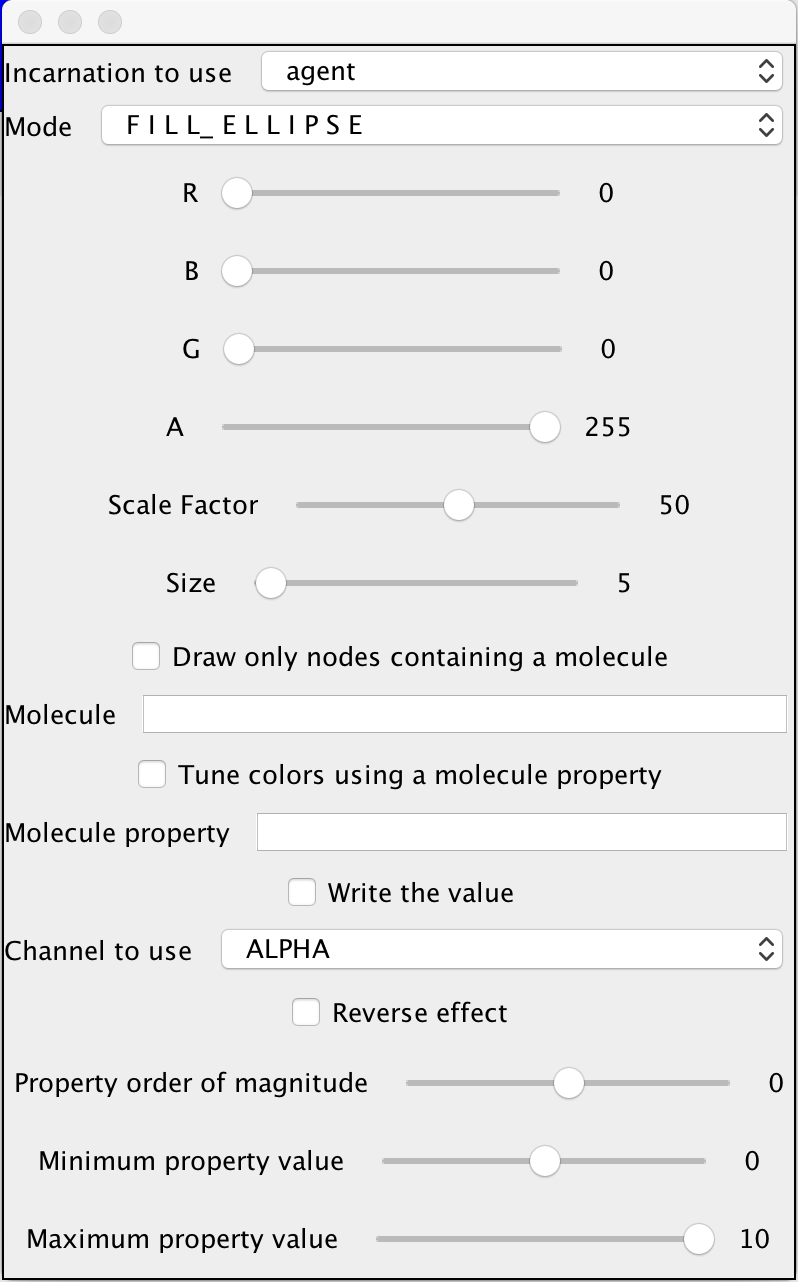
\includegraphics[width=6cm]{images/tematizzazioneSimulazione.png} % inserisce una figura larga 12.5cm
% inserisce la legenda ed etichetta la figura con \label{fig:prima}
\caption[Stile della simulazione]{Stile della simulazione} \label{fig:tematizzazioneSimulazione}
\end{center}
\end{figure}

Dall'immagine si può osservare che l'effetto può essere composto da molteplici fattori.
Per quanto riguarda lo stile scelto per questa simulazione sono stati utilizzati i controlli presenti nella metà superiore della finestra.

\paragraph*{}
Sono state definite delle stringhe identificative per le molecole che si riferiscono univocamente ai vari ruoli nella scena: minatore (miner), miniera (goldmine), deposito (deposit), pepita (nugget).
Per ogni stringa è stato creato un relativo stile definito da un colore (tramite il modello RGBA), un fattore di scala e una dimensione per rappresentare il nodo.

L'associazione tra ogni effetto e la rispettiva molecola viene realizzato spuntando la casella di controllo relativa a \textit{`Draw only nodes containing a molecule'} ed inserendo nella casella di testo sottostante la stringa identificativa della molecola che si vuole abbinare.

\paragraph*{}
Nell'implementazione dell'interprete sono opportunamente create le molecole utilizzando la classe SimpleMolecule, passando come parametro identificativo le stringhe descritte poco sopra. Gli oggetti istanziati sono poi inseriti all'interno del nodo.

Una volta creato lo stile desiderato è possibile salvarlo (viene generato un file con estensione .aes) in modo da poterlo riutilizzare.
All'avvio di una simulazione di default non è presente nessuno stile però è possibile caricare un file salvato in precedenza.
Lo stile non è necessario al fine dell'esecuzione della simulazione ma è molto utile per poter comprendere al meglio il comportamento degli agenti nell'avanzamento della simulazione.


\section{Implementazione agenti}
L'agente, come già accennato in precedenza, è composto e definito tramite due parti:
\begin{itemize}
\item la \textbf{teoria} che definisce come e a quali eventi reagire in base ad un contesto;
\item la \textbf{classe} che definisce in che modo i comportamenti sono trasmessi dall'interprete alla teoria.
\end{itemize}
In questa sezione sono descritte le teorie e le classi degli agenti che sono stati implementati per la realizzazione dello scenario di test.

\subsection{Miniera -- Goldmine}
La miniera è un'entità che è posizionata in modo casuale all'interno dell'ambiente, che mantiene la sua posizione nel tempo e che contiene delle risorse.
Data questa descrizione la sua realizzazione è stata subito associata agli spazi di tuple. Si è quindi implementata la classe Goldmine estendendo la classe AbstractSpatialTuple.

Per iniziare è stata scritta la teoria dell'agente in cui è definito il suo comportamento e solo successivamente è stata implementata la classe all'interno dell'interprete e le relative funzionalità.

\subsubsection{Teoria tuProlog miniera}
La teoria di questo agente è poco complessa poichè definisce solamente il caricamento di un numero casuale di risorse (ovvero le pepite) sotto forma di tuple all'interno dello spazio di tuple.

\switchToProlog{}
\begin{lstlisting}[float,firstnumber=1,label={lst:Goldmine},caption={Teoria miniera}]
init :-
    agent <- generateNextRandom returns RAND,
    NUGGETS is RAND * 1.0,
    loadNuggets(NUGGETS).

loadNuggets(NUGGETS) :-
    NUGGETS > 0,
    assertz(nugget),
    N is NUGGETS - 1,
    loadNuggets(N).

loadNuggets(NUGGETS) :-
    NUGGETS < 0,
    agent <- setConcentration.
\end{lstlisting}

Nel corpo della regola $init$ viene inizialmente recuperato un numero random, attraverso l'invocazione del metodo $generateNextRandom()$ definito nell'agente, che rappresenta le pepite da posizionare all'interno della miniera.
Il caricamento delle risorse viene fatto tramite l'invocazione della regola $loadNuggets(NUGGETS)$ con la quale sono inseriti i fatti nello spazio di tuple: se le risorse sono state tutte caricate viene invocato il metodo $setConcentration()$, definito appositamente all'interno dell'agente, che viene utilizzato per impostare le molecole per lo stile grafico dello spazio di tuple nella simulazione.

\subsubsection{Implementazione classe miniera}
Per quanto riguarda la classe della miniera si è deciso, come detto poco sopra, di utilizzare lo spazio di tuple. La classe astratta AbstractSpatialTuple definisce al suo interno la struttura base dello spazio di tuple e le funzioni per eseguire i suoi comportamenti caratteristici $in$, $rd$ e $out$, rispettivamente trasformati nelle azioni $writeTuple$, $readTuple$, $takeTuple$.
Per definire la miniera è stata quindi definita la classe Goldmine che estende la classe astratta implementando quindi un semplice spazio di tuple.
Oltre ad essere uno spazio di tuple, la classe però implementa anche la super classe astratta AbstractAgent che fa essere Goldmine anche un agente: è quindi necessario implementare all'interno della classe anche i metodi $execute()$ e $cloneAction(node, reaction)$. Il primo di questi due metodi è quello più importante, poichè definisce in che modo lo spazio di tuple opererà nel suo ciclo di ragionamento permettendo a quest'ultimo di reagire alle richieste ricevute.

Per lo stile all'interno della simulazione è stato implementato il metodo $setCon\-cen\-tra\-tion()$. Questo metodo, come già accennato nella sezione precedente, viene utilizzato per inserire un oggetto molecola nel nodo, la quale è utilizzata per lo stile della simulazione. La molecola viene creata ed inserita con le istruzioni presenti nel Codice sorgente \ref{lst:CreazioneInserimentoMolecola} solo dopo aver verificato che nella teoria dell'agente sono effettivamente presenti delle risorse.

\switchToJava{}{}
\begin{lstlisting}[float,firstnumber=1,label={lst:CreazioneInserimentoMolecola},caption={Creazione e inserimento molecola}]
SimpleMolecule sm = new SimpleMolecule("nugget");
this.getNode().setConcentration(sm, 0);
\end{lstlisting}
La stringa `nugget' è quella che deve essere inserita nella casella di testo a fianco dell'etichetta Molecule nella Figura \ref{fig:tematizzazioneSimulazione} e che deve essere abilitata cliccando la checkbox appena sopra.

\paragraph*{}

Per via della necessità di associare uno stile alla simulazione, si è dovuto sovrascrivere il metodo dello spazio di tuple relativo alla funzionalità $out$, o $takeTuple$.
Qui di seguito è descritta la funzionalità già implementata nella classe astratta. Nel paragrafo successivo viene invece riportata la modifica effettuata per definire lo stile della miniera all'interno della simulazione.

Nell'implementazione della funzionalità già definita all'interno della classe astratta, la procedura è la seguente:
\begin{enumerate}
\item recupero di una tupla che corrisponda al template tramite il predicato $retract$;
\item interrogazione per ottenere dal termine estratto il template popolato con i valori recuperati;
\item invio del template popolato tramite un messaggio all'agente che lo aveva richiesto.
\end{enumerate}
Nel caso l'operazione di recupero della tupla non vada a successo quella richiesta viene aggiunta tra quelle in attesa, le quali, se previsto nel ciclo di ragionamento, periodicamente vengono verificate nuovamente per poter essere completate.
Nel caso in cui la richiesta del template è andata a successo e questa è presente nell'elenco di quelle in attesa allora la stessa viene rimossa prima di procedere con l'operazione indicata nell'elenco con il numero 2.

La modifica effettuata è relativa solamente allo stile, cioè all'inserimento o alla rimozione di un oggetto molecola, e quindi la funzionalità principale rimane quella appena descritta.
Il codice aggiunto è stato inserito prima di effettuare l'operazione di invio del messaggio all'agente. L'aggiunta consiste in un'interrogazione per verificare se dopo aver estratto una risorsa ci sono ancora pepite, presenti nella teoria sotto forma di fatti, all'interno della miniera. In caso affermativo viene lasciata la molecola che era stata impostata precedentemente invocando dalla teoria la funzionalità $setConcentration()$. Diversamente, se non sono più presenti risorse nella miniera la molecola viene rimossa e, se lo stile della simulazione è opportunamente configurata, il cambiamento porterà ad una modifica visiva del nodo.

\subsection{Minatore -- Miner}
Il minatore è l'agente con il comportamento più complesso per lo scenario preso in esempio.
Il suo compito è quello di muoversi nell'ambiente cercando miniere da cui estrarre risorse da portare al deposito.
Il comportamento del minatore è stato scomposto in 4 fasi o stati:
\begin{enumerate}
\item harvesting: spostamento casuale e ricerca di risorse all'interno di miniere;
\item toDeposit: recuperata la pepita, spostamento verso il deposito per consegnarla;
\item toMine: depositata la pepita, ritorno alla miniera;
\item arrivato alla miniera torna nello stato harvesting.
\end{enumerate}

\subsubsection{Teoria tuProlog minatore}
Le fasi descritte sono state poi riportate all'interno della teoria dell'agente, mostrata nel Codice sorgente \ref{lst:Goldmine}, per definirne il comportamento in relazione agli eventi innescati dall'interprete. Le invocazioni evidenziate in blu sono relative a regole definite all'interno della teoria dell'agente e che non sono state mostrate.

Le regole $ randomDirection(D)$ e $randomSpeed(S)$ restituiscono nella variabile passata, rispettivamente $D$ e $S$, il valore ottenuto dall'invocazione combinata delle funzioni definite all'interno della classe AbstractAgent, e quindi disponibile in tutte le implementazioni di un agente, che generano un valore random e lo applicano alla distribuzione di Levy.

La regola $handlePosition$ si occupa, in modo molto simile a quello che viene fatto nella regola $init$, di generare una nuova velocità e un delta per la direzione da impostare nel nodo, mentre $changeDirection(X,Y)$ modifica solamente la direzione calcolando il valore corretto per raggiungere il punto (X,Y) data la posizione corrente.

La regola $checkMineDistance$ definisce la guardia che verifica che l'agente, dopo aver consegnato la pepita al deposito e essersi diretto alla miniera, è effettivamente arrivato a destinazione e può tornare nello stato `harvesting'.

\switchToProlog{}
\lstset{
  keywordstyle=\color{blue},
  morekeywords={randomDirection,randomSpeed,handlePosition,changeDirection,checkMineDistance}
}
\medskip
\begin{lstlisting}[float,firstnumber=1,label={lst:Miner},caption={Teoria minatore}]
init :-
    addBelief(deposit(2,2)),
    addBelief(harvesting),
    randomDirection(D),
    randomSpeed(S),
    node <- changeNodeSpeed(S),
    node <- changeDirectionAngle(D).

%(1)
'<-'(onAddBelief(position(X,Y)), [belief(harvesting)], [handlePosition, takeTuple(nugget)]).

%(4)
'<-'(onAddBelief(position(X,Y)), [checkMineDistance(X,Y,MX,MY)], [removeBelief(mine(_,_)), removeBelief(toMine), addBelief(harvesting), changeDirection(MX,MY)]).

%(2)
'<-'(onResponseMessage(msg(nugget,X,Y)), [removeBelief(harvesting)], [addBelief(toDeposit), addBelief(mine(X,Y)), belief(deposit(DX,DY)), changeDirection(DX,DY)]).

%(3)
'<-'(onAddBelief(distance(deposit,ND)), [removeBelief(toDeposit)], [iSend(deposit,nugget), addBelief(toMine), belief(mine(X,Y)), changeDirection(X,Y)]).
\end{lstlisting}

Nella fase di configurazione iniziale, regola $init$, vengono impostati all'interno della teoria del minatore il belief relativo alla posizione del deposito e quello relativo allo stato iniziale dell'agente, `harvesting'. Successivamente sono generati i valori per direzione e velocità che poi sono impostati nel nodo.

Dopo la regola $init$ sono descritti i fatti che definiscono il comportamento dell'agente, mostrato ad inizio sezione, e che gli permettono di reagire al verificarsi di opportuni eventi.
I fatti seguono la seguente struttura $\leftArrow(EVENT, GUARD, BODY).$, dove $EVENT$ è l'evento al quale l'agente vuole reagire, $GUARD$ identifica il contesto o la condizione per cui le azioni contenute nel $BODY$ possano essere eseguite.

I fatti identificati dalle fasi 1 e 4 agiscono entrambi in relazione all'evento di aggiornamento della posizione. Il contesto della fase 1 è relativo allo stato `harvesting' mentre quello della fase 4 è la vicinanza del nodo che contiene l'agente rispetto alla miniera che deve raggiungere.
Gli altri due contesti, relazionati ad eventi quali la ricezione di un messaggio dallo spazio di tuple e l'aggiornamento della distanza dal nodo contenente l'agente deposito, sono associati alla rimozione di un certo stato che quindi risulta bloccante finchè lo stato da rimuovere non è presente all'interno della `belief base' dell'agente.

Tra le azioni definite nei corpi dei vari fatti una spiegazione la merita l'utilizzo del belief $mine(X,Y)$. Questo viene utilizzato per salvare la posizione della miniera da cui è stata recuperata l'ultima risorsa, prima di andare al deposito per consegnarla, in modo tale da poter tornare direttamente alla miniera, una volta depositata la pepita, per continuare ad estrarre risorse risultando più veloce ed efficace.

\subsubsection{Implementazione classe minatore}
Per quanto riguarda la parte lato interprete relativa all'agente minatore è stata utilizzata la classe SimpleAgent che estende da AbstractAgent. Questa classe rappresenta un esempio di come può essere immediata l'implementazione di un agente, che racchiude tutte le funzionalità principali, a partire da quello che è già stato prodotto e mostrato precedentemente in questo documento.

\switchToJava{}{}
\begin{lstlisting}[float,firstnumber=1,label={lst:SimpleAgentReasoningCycle},caption={Ciclo di ragionamento per l'agente completo}]
@Override
public void execute() {
    if (this.isInitialized()) {
        //Agent's reasoning cycle
        
        this.beliefBaseChanges();
        this.readMessage();

        // SpatialTuples extension
        this.retrieveTuples();

        this.executeIntention();
    } else {
        this.initializeAgent();
        this.initReasoning();
    }
}
\end{lstlisting}

Per implementare la classe SimpleAgent (denominata in questo modo perchè implementa un agente con tutte le funzionalità principali) è stato sufficiente implementare il costruttore, richiamando quello di AbstractAgent, e i due metodi $cloneAction(node, reaction)$ e $execute()$.
Nel Codice sorgente \ref{lst:SimpleAgentReasoningCycle} è mostrato come è stato definito il ciclo di ragionamento.
Come si può notare è stata utilizzata una condizione, che utilizza un flag definito nella classe astratta, per determinare se l'agente è stato inizializzato, ovvero se ha completato la configurazione iniziale.

Nel primo ciclo di ragionamento avviene appunto la configurazione iniziale. La prima funzione che viene chiamata è $initializeAgent()$ che termina la configurazione utilizzata dall'interprete, e all'interno della quale viene modificato il flag citato in precedenza, e poi viene invocata $initReasoning()$ che esegue quanto previsto dalla regola $init$ se presente nella teoria dell'agente.

Dal ciclo di ragionamento successivo vengono eseguite le funzioni per:
\begin{enumerate}
\item controllare le modifiche alla `belief base';
\item leggere i messaggi ricevuti;
\item inviare le richieste agli spazi di tuple;
\item eseguire un'intenzione.
\end{enumerate}
La funzione $beliefBaseChanges()$ recupera tutte le modifiche effettuate alla `belief base' e, per ognuna per cui esiste un comportamento nella teoria, genera un'intenzione inserita opportunamente nella teoria. In modo simile, $readMessage()$ recupera, se presente, un messaggio dalla lista di quelli in entrata e, anche in questo caso, se nella teoria è previsto un comportamento viene generata un'intenzione.

La funzione $retrieveTuples()$ recupera ed invia immediatamente tutte le richieste agli spazi di tuple opportuni.
Per concludere viene invocata la funzione $executeIntention()$ che sceglie un'intenzione tra quelle presenti all'interno dell'agente (il metodo di selezione è Round-Robin), la esegue e poi la inserisce in coda alla lista delle intenzioni.

\subsection{Deposito -- Deposit}
Per quanto riguarda il deposito, il suo compito è semplicemente quello di raccogliere le risorse consegnate dai minatori.
Nella soluzione proposta il deposito è stato implementato da un agente ma, come detto nell'introduzione del capitolo, è possibile realizzare simulazioni con un'implementazione diversa.

\subsubsection{Teoria tuProlog deposito}
Per quanto riguarda la teoria del deposito non è necessario definire alcun piano poichè esso non ha compiti se non quello di accettare le risorse ricevute. Si è quindi definita una teoria contenente una regola $init$ vuota (ovvero che ha come unica istruzione del corpo `true').

\subsubsection{Implementazione classe deposito}
La classe utilizzata per rivestire questo ruolo all'interno della simulazione è anche in questo caso la classe SimpleAgent poichè è un'implementazione di un agente completo già pronta per essere utilizzata.
%
Le funzionalità disponibili sono sicuramente maggiori rispetto a quelle che sono effettivamente utilizzate ma, data la struttura già fornita della classe astratta, questo non impatta sull'efficienza e rimane molto semplice da utilizzare.

\section{Configurazione della simulazione}
Per definire la simulazione si deve scrivere un'opportuna configurazione nella quale sono descritti, attraverso le keyword, quali oggetti utilizzare nella simulazione in relazione al modello creato. Nel Codice sorgente \ref{lst:GoldminersSimulation} sono mostrate e descritte in dettaglio le varie parti che compongono la configurazione e che sono state precedentemente spiegate nella sezione \ref{sctn:ScrivereUnaSimulazione}.

\switchToProlog{}
\begin{lstlisting}[float,firstnumber=1,label={lst:GoldminersSimulation},caption={Configurazione simulazione Goldminers}]
incarnation: agent

network-model:
  type: ConnectWithinDistance
  parameters: [2]

displacements:
  - in: {type: Circle, parameters: [2,2,2,0.2]}
    programs:
      -
        - time-distribution: 9
          program: "miner"

  - in: {type: Circle, parameters: [1,2,2,0.2]}
    programs:
      -
        - time-distribution: 9
          program: "deposit"

  - in: {type: Circle, parameters: [1,2,2,0.2]}
    programs:
      -
        - time-distribution: 9
          program: "postman"

  - in: {type: Circle, parameters: [10,2,2,5]}
    programs:
      -
        - time-distribution: 9
          program: "goldmine"
\end{lstlisting}

La prima cosa che si può notare nella configurazione è la specifica dell'incarnazione utilizzata `agent', ovvero quella definita per questo progetto.

Il secondo parametro impostato in configurazione è il `network-model', il parametro che definisce la `linking-rule', che descrive in che modo ogni nodo presente all'interno dell'ambiente è collegato con gli altri. Attraverso questa regola cambia il numero di nodi presenti nel vicinato di ogni nodo. Nel caso specifico, è stato scelto di utilizzare una classe che utilizza la relazione di distanza per collegare i vari nodi ed alla quale è stato passato come parametro il valore 2; per ogni nodo, sono considerati suoi vicini tutti i nodi che ad ogni istante della simulazione siano posizionati all'interno di un cerchio di dimensione 2 il cui centro è il nodo stesso.

Il terzo ed ultimo parametro è `displacements' che definisce una lista con la disposizione dei nodi ed il loro contenuto.
%
La lista si compone di due keyword: $in$ e $programs$. La prima richiede un oggetto che definisce il tipo della geometria e i parametri per costruirla, mentre la seconda utilizza un'ulteriore lista all'interno della quale sono definite le reazioni associate ad ogni nodo.

Per tutti i ruoli della scena è stato utilizzato il cerchio come geometria per posizionare i nodi, passando per ognuno dimensioni e quantità di nodi differenti.

Attraverso la keyword $program$ si definiscono le reazioni che saranno inserite nei nodi: come si può notare dalla configurazione, per ogni nodo è stata definita una sola reazione.
Per definire una reazione sono stati utilizzati una distribuzione temporale ed una stringa; quest'ultima sarà poi utilizzata durante la creazione di istanze della classe AgentReaction e con la quale verrà istanziata all'interno della reazione la classe dell'agente relativa.

Come parametro della distribuzione temporale è stato scelto 9: questo valore ha consentito, anche in base al valore di distribuzione temporale associato all'azione di spostamento posizionata in maniera intrinseca nel nodo, di ottenere un comportamento fluido durante l'esecuzione della simulazione.


\section{Metriche di progetto}
Le metriche di progetto rappresentano un insieme di indicatori per tenere sotto controllo e prevedere l'andamento delle principali variabili del progetto (costi, tempi, qualità, risorse).
Le metriche includono solitamente una serie di indicatori standard ma ne possono essere aggiunti altri \textit{ad hoc} in relazione al progetto.

Con le metriche è possibile quantificare in modo obiettivo le performance del progetto misurando gli indicatori predisposti. L'uso principale delle metriche è quello di misurare l'avanzamento del progetto. Il loro utilizzo permette di identificare i problemi di costo/schedulazione prima che diventino criticità e aiutare a focalizzarsi sul completamento delle attività.

\subsection{Metriche software del progetto}
Con le metriche di progetto si misura il codice, quindi è possibile analizzare solamente la parte del lavoro di tesi relativa all'implementazione dell'interprete del linguaggio all'interno del simulatore Alchemist.
La figura \ref{fig:codeMetrics} è stata ottenuta tramite l'utilizzo del plugin CodeMR Metrics disponibile nell'IDE IntelliJ IDEA. Inoltre, è stato utilizzato anche il plugin Statistics per avere un dettaglio maggiore per quanto riguarda le SLOC.
%crea l'ambiente figura;
\begin{figure} % [h] sta per here, cioè la figura va qui
\begin{center} % centra nel mezzo della pagina la figura
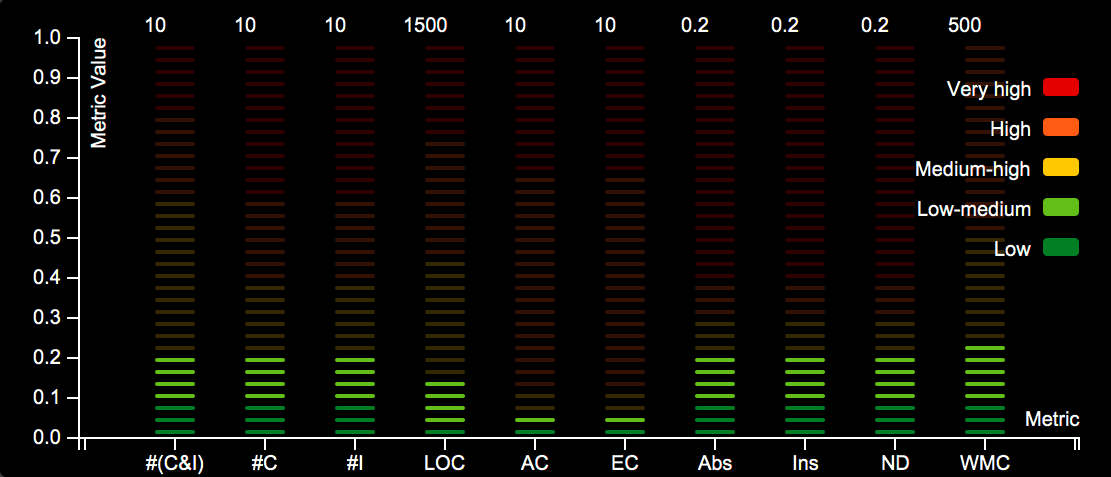
\includegraphics[width=13cm]{images/codeMetrics.png} % inserisce una figura larga 12.5cm
% inserisce la legenda ed etichetta la figura con \label{fig:prima}
\caption[Metriche di progetto]{Metriche di progetto} \label{fig:codeMetrics}
\end{center}
\end{figure}

\paragraph*{}
Per la realizzazione dell'incarnazione ad agenti all'interno di Alchemist sono state definite dieci classi Java per implementare la struttura e mostrare come creare le diverse tipologie di agenti. Il totale delle righe presenti all'interno dei file è 2.085, di cui 1.109 sono SLOC e 751 sono di documentazione.
In questo numero non sono calcolate, come accennato precedentemente, le righe scritte per la definizione delle teorie degli agenti utilizzate per la realizzazione degli scenari di test.

La complessità ciclomatica è utilizzata per misurare la complessità di un programma misurando il numero di cammini linearmente indipendenti attraverso il grafo di controllo di flusso.
L'incarnazione realizzata all'interno di Alchemist ha un valore totale di complessità ciclomatica pari a 220, con una media di 2.10.
%crea l'ambiente figura;
\begin{figure} % [h] sta per here, cioè la figura va qui
\begin{center} % centra nel mezzo della pagina la figura
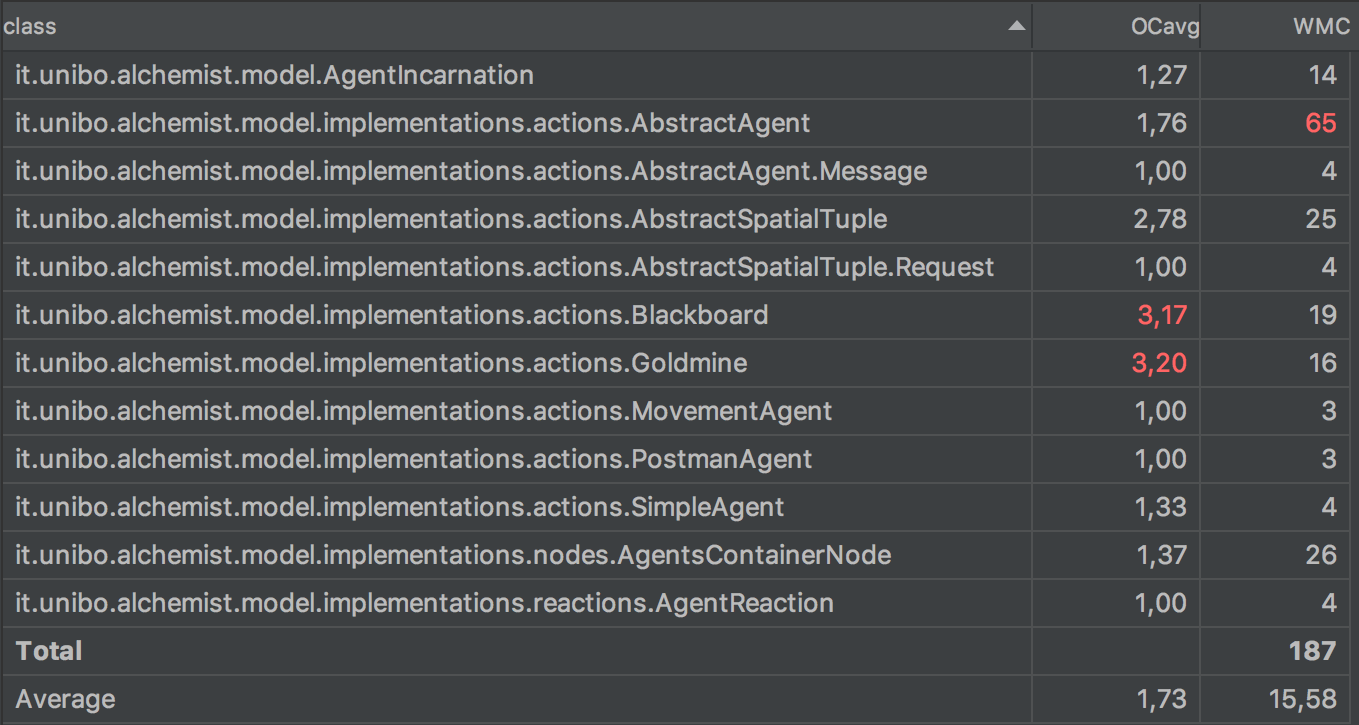
\includegraphics[width=14cm]{images/complessitaCiclomatica.png} % inserisce una figura larga 12.5cm
% inserisce la legenda ed etichetta la figura con \label{fig:prima}
\caption[Complessità ciclomatica]{Complessità ciclomatica} \label{fig:cyclomaticComplexity}
\end{center}
\end{figure}

Nell'immagine \ref{fig:cyclomaticComplexity} è mostrato in dettaglio la complessità ciclomatica delle varie classi, anche quelle innestate, implementate all'interno dell'incarnazione, misurata utilizzando il plugin MetricsReloaded disponibile nell'IDE IntelliJ IDEA. Per ogni classe viene descritto il valore relativo alla complessità operazionale media (OCavg) e quello relativo alla complessità totale(WMC).
La complessità ciclomatica totale dell'incarnazione è 187, la cui media ripartita tra le viarie classi è 15.58.
Si può notare fin da subito che la classe AbstractAgent, la quale definisce tutte le funzionalità di base dell'agente, risulti essere di una complessità ben maggiore rispetto a tutte le altre classi, seguita dalla classe del nodo e poi da quelle che utilizzano il modello Spatial Tuples.
Proprio tra quest'ultime, nello specifico Blackboard e Goldmine che sono due implementazioni della classe AbtractSpatialTuple, sono presenti le classi con una compkessità ciclomatica media più alta. Questa caratterizzazione può essere spiegata dal fatto che per definire gli spazi di tuple, vista l'ereditarietà dalla classe AbstractAgent, è stato necessario implementare le funzionalità di gestione dello spazio di tuple, nella classe AbstractSpatialTuple, o nuove personalizzazioni della funzionalità base, nelle implementazioni specifiche degli spazi di tuple.

Per quanto riguarda i metodi presenti all'interno delle varie classi non è mostrato il dettaglio ma sono riportati soltanto i valori totali.
La complessità ciclomatica essenziale, ev(G), è 117, la complessità di design, iv(G), è 213 mentre la complessità ciclomatica totale, v(G), è 220.


\chapter{Conclusioni}\label{chap:conclusions}
Con questo lavoro di tesi è stato definito un nuovo linguaggio per la programmazione ad agenti basato sulla struttura del modello di AgentSpeak al quale è stato integrata la gestione del ragionamento degli agenti proposta dall'interprete Jason.
%
Il linguaggio definito permette di scrivere teorie tuProlog per implementare il comportamento degli agenti sfruttando gli eventi e i predicati messi a disposizione.
Questo linguaggio non si occupa di gestire la piattaforma sulla quale opereranno gli agenti ma solo di dare una definizione degli elementi che permetteranno all'agente di essere autonomo, reattivo e proattivo.

L'interprete di questo linguaggio potrà essere implementato in qualsiasi ambiente, da quello reale a quello simulato, poichè grazie all'utilizzo della libreria tuProlog sarà possibile realizzare efficientemente la gestione delle interazioni con le primitive del nuovo linguaggio.
%
Per l'interprete quindi sarà necessario implementare un applicativo che gestisca lo scheduling degli eventi, in caso di ambiente simulato, o la comunicazione con i percettori, in caso di ambiente reali, e trasmetta le informazioni alla teoria dell'agente utilizzando il linguaggio attraverso la libreria tuProlog.

All'interno del lavoro di tesi è descritto come è stato realizzato un interprete per il linguaggio utilizzando il simulatore Alchemist.
Con questo esempio, anche attraverso alla flessibilità del meta-modello di Alchemist, si è mostrata la grande capacità di adattamento del linguaggio e la trasparenza con cui l'interprete può gestire gli eventi e gli agenti. 

\section{Vantaggi approccio scelto}
Il linguaggio è stato realizzato con l'obiettivo di fornire una nuova prospettiva più snella e dinamica che permetta di portare la potenza del modello ad agenti su varie piattaforme cercando di semplificare il lavoro di integrazione e di implementazione con questo modello.

Attraverso il linguaggio definito in questo lavoro è possibile portare il modello ad agenti da un ambiente simulato, come l'interprete che è stato realizzato all'interno di questo progetto di tesi, ad un ambiente reale, realizzando ad esempio un applicativo per dispositivi mobile ognuno dei quali esegue degli agenti, i quali comunicano con altri agenti presenti in differenti device.

%-----------------------------------------
%-----------------------------------------

\backmatter	

\bibliographystyle{plain}
\bibliography{bibtex.bib}



% non numera l'ultima pagina sinistra
%\clearpage{\pagestyle{empty}\cleardoublepage}
%\chapter{Ringraziamenti}
%\thispagestyle{empty}
%Contenuto ringraziamenti
\end{document}
